
\documentclass[letterpaper,oneside]{book}%

\usepackage[left=1in,right=2.75in,top=1in,bottom=1in]{geometry}
\marginparwidth 1.75in

\usepackage{tabls}
\usepackage{booktabs}
\usepackage{amsmath}
\usepackage{amssymb}
\usepackage{amsthm}
\usepackage{amsfonts}
\usepackage{multicol}
\usepackage{enumitem}
\usepackage{microtype}
\usepackage{tikz}
\usetikzlibrary{positioning}

\newcommand{\wrapup}{
\bmw{\section{Wrap Up}
Once you have finished the problems in the section and feel comfortable with the ideas, create a short one page lesson plan that contains examples of the key ideas.  You will get a chance to teach from this lesson plan prior to taking the exam. Then log on to Brainhoney and download the quiz. Once you have taken the quiz, you can upload your work back to brainhoney and then download the key to see how you did. If you still need to work on mastering some of the ideas, please do so and then demonstrate your mastery though the quiz corrections.}
}
\newcommand{\myscale}{1}

\usepackage{graphicx}
\usepackage{wrapfig}

\newcommand{\ds}{\displaystyle}
\newcommand{\dfdx}[1]{\frac{d#1}{dx}}
\newcommand{\ddx}{\frac{d}{dx}}


\let\oldmarginpar\marginpar
\renewcommand\marginpar[1]{\-\oldmarginpar{\raggedright\footnotesize #1}}
%\renewcommand\marginpar[1]{\-\oldmarginpar[\raggedleft\footnotesize #1]{\raggedright\footnotesize #1}}

\renewcommand{\thefootnote}{\roman{footnote}}
\newcommand{\note}[1]{\footnote{#1}\marginpar{\fbox{\textbf{\thefootnote}}}}
%%%%%%%To make all notes ignored, uncomment the following command.
\renewcommand{\note}[1]{}

%\usepackage[12hr]{datetime}
%\newdateformat{draftdate}{%
%\shortdayofweekname{\THEDAY}{\THEMONTH}{\THEYEAR}, %
%\THEDAY\ \shortmonthname[\THEMONTH] \THEYEAR}
%\draftdate
%\usepackage{eso-pic}
%\AddToShipoutPicture{\put(10,10){\small Draft: \today\ at \currenttime }}%--- version: \MakeUppercase{\svnInfoRevision}}}

\newcommand{\bmw}[1]{}
\newcommand{\marginparbmw}[1]{}
\newcommand{\marginparlarsonfive}[1]{\marginpar{#1}}

\theoremstyle{plain}
\newtheorem{theorem}{Theorem}[chapter]
\newtheorem*{theorem*}{Theorem}
\newtheorem{lemma}[theorem]{Lemma}
\newtheorem*{lemma*}{Lemma}
\newtheorem{proposition}[theorem]{Proposition}
\newtheorem{corollary}[theorem]{Corollary}

\newtheoremstyle{box}%
{}{}% standard spacing before and after
{}% Body style
{}{\bfseries}{.}% Heading indent, font, and punctuation
{ }% space after heading
{\thmname{#1}\thmnumber{ #2}\thmnote{: #3}}% head spec

\newtheoremstyle{problem}%
{}{}% standard spacing before and after
{}% Body style
{}{\bfseries}{}% Heading indent, font, and punctuation
{1em}% space after heading
{\fbox{\thmname{#1}\thmnumber{ #2}\thmnote{: #3}}}% head spec

\theoremstyle{box}
\newtheorem{definition}[theorem]{Definition}
\newtheorem{dfn}[theorem]{Definition}
\newtheorem*{definition*}{Definition}
\newtheorem{observation}[theorem]{Observation}
\newtheorem{remark}[theorem]{Remark}
\newtheorem{example}[theorem]{Example}
\newtheorem{prb}[theorem]{Problem}
\newtheorem{question}[theorem]{Question}
\newtheorem*{prep-problems}{Preparation Problems}

%\newtheorem{problem}[theorem]{Problem}
\theoremstyle{problem}
\newtheorem{problemnum}[theorem]{Problem}
\newenvironment{problem}[1][]{\begin{problemnum}[#1]}{\end{problemnum}\hrule\bigskip}

% Abbreviations
\newcommand{\ii}{\ensuremath{\vec \imath}}
\newcommand{\jj}{\ensuremath{\vec \jmath}}
\newcommand{\kk}{\ensuremath{\vec k}}
\newcommand{\vv}{\ensuremath{\mathbf{v}}}
\newcommand{\colvec}[1]{\ensuremath{\begin{bmatrix}#1\end{bmatrix}}}
\DeclareMathOperator{\rank}{rank}
\DeclareMathOperator{\rref}{rref}
\DeclareMathOperator{\vspan}{span}
\DeclareMathOperator{\trace}{tr}
\DeclareMathOperator{\proj}{proj}
\DeclareMathOperator{\curl}{curl}
\newcommand{\RR}{\ensuremath{\mathbb{R}}}
% \vp is "vector prime" and corrects spacing when doing something like
% $\vec r'$ (which has the vector and prime almost touching).
% Instead, do something like $\vec r\vp$
\newcommand{\vp}{\ensuremath{^{\,\prime}}}


%%% Local Variables: 
%%% mode: latex
%%% TeX-master: t
%%% End: 

%The purpose of this code is to allow me to put lines in matrices so that I can create augmented matrices.
\makeatletter
\renewcommand*\env@matrix[1][*\c@MaxMatrixCols c]{%
  \hskip -\arraycolsep
  \let\@ifnextchar\new@ifnextchar
  \array{#1}}
\makeatother

\newcommand{\cl}[1]{  \begin{matrix}  #1  \end{matrix}  }
\newcommand{\bm}[1]{  \begin{bmatrix}  #1  \end{bmatrix}  }
\newcommand{\inv}{^{-1}}
\newcommand{\im}{\ensuremath{\text{im }}}
\newcommand{\R}{\mathbb{R}}

%------------------------------------------------------------------------------------------------------------

\usepackage{hyperref}


\begin{document}
\frontmatter
\title{Multivariable Calculus}
\author{Ben Woodruff\thanks{Mathematics Faculty at Brigham Young
    University--Idaho, \url{woodruffb@byui.edu}}}
\date{Typeset on \today\\
\vfill
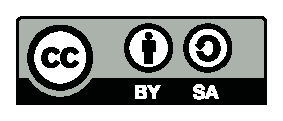
\includegraphics[height=1.3cm]{by-sa}
\vfill}
\maketitle
\thispagestyle{empty}
\noindent\copyright{ 2012 Ben Woodruff.  Some Rights Reserved.\\

\bigskip

\noindent This work is licensed under the Creative Commons Attribution-Share Alike 3.0 United States License.  You may copy, distribute, display, and perform this copyrighted work, but only if you give credit to Ben Woodruff, and all derivative works based upon it must be published under the Creative Commons Attribution-Share Alike 3.0 United States License. Please attribute this work to Ben Woodruff, Mathematics Faculty at Brigham Young University--Idaho, \url{woodruffb@byui.edu}. To view a copy of this license, visit
\begin{center}
  \url{http://creativecommons.org/licenses/by-sa/3.0/us/}
\end{center}
or send a letter to Creative Commons, 171 Second Street, Suite 300, San Francisco, California, 94105, USA.}
\tableofcontents

\mainmatter

\chapter{Review}
This unit covers the following ideas. In preparation for the quiz and exam, make sure you have a lesson plan containing examples that explain and illustrate the following concepts.  \begin{enumerate}
\item Give a summary of the ideas you learned in 112, including graphing, derivatives (product, quotient, power, chain, trig, exponential, and logarithm rules), and integration ($u$-sub and integration by parts).
\item Compute the differential $dy$ of a function and use it to approximate the change in a function. 
\item Explain how to perform matrix multiplication and compute determinants of square matrices.
\item Illustrate how to solve systems of linear equations, including how to express a solution parametrically (in terms of $t$) when there are infinitely solutions.
\item Extend the idea of differentials to approximate functions using parabolas, cubics, and polynomials of any degree (in other words, using Taylor polynomials).
\end{enumerate}
You'll have a chance to teach your examples to your peers prior to the exam.

%\section{Preparation and Suggested Homework}
%
%\begin{center}
%\begin{tabular}{ll}
%&Preparation Problems\\
%\hline\hline
%Day 1 & 1e, 3a, 2g, 2c
%\\\hline
%Day 2 & 1f, 3b, 3d, 4a
%\\\hline
%Day 3 & 4e, 5h, 6b, 6e
%\\\hline
%\end{tabular}
%\end{center}

\section{Review of First Semester Calculus}

\subsection{Graphing}
We'll need to know how to graph by hand some basic functions. If you have not spent much time graphing functions by hand before this class, then you should spend some time graphing the following functions by hand. When we start drawing functions in 3D, we'll have to piece together infinitely many 2D graphs.  Knowing the basic shape of graphs will help us do this.
\begin{problem}
Provide a rough sketch of the following functions, showing their basic shapes:
$$\displaystyle x^2, x^3, x^4, \frac{1}{x}, \sin x, \cos x, \tan x, \sec x, \arctan x, e^x,\ln x.$$ 
Then use a computer algebra system, such as \href{http://http://www.wolframalpha.com/}{Wolfram Alpha}, to verify your work. I suggest Wolfram Alpha, because it is now built into Mathematica 8.0.  If you can learn to use Wolfram Alpha, you will be able to use Mathematica.
\end{problem}


\subsection{Derivatives}
In first semester calculus, one of the things you focused on was learning to compute derivatives. You'll need to know the derivatives of all the basic functions (found on the end cover of almost every calculus textbook). Being able to compute derivatives accurately and rapidly will help make learning calculus in high dimensions much easier (as every derivative will involve multiple derivatives).

The following rules are crucial.
\begin{itemize}
\item Power rule {$(x^n)' = nx^{n-1}$}
\item Sum and difference rule {$(f\pm g) = f'\pm g'$}
\item Product {$(fg)' = f' g + fg'$} and quotient rule  {$\ds\left(\frac f g\right)' = \frac{f' g - fg'}{g^2}$}
\item Chain rule (arguably the most important) {$(f\circ g)' = f'(g(x))\cdot g'(x)$}
\end{itemize}

\begin{problem}
\marginpar{\bmw{See sections 3.2-3.6 for more practice with derivatives. The later problems in 3.6 review of most of the entire differentiation chapter.}}
Compute the derivative of $e^{\sec x}\cos(\tan(x)+\ln(x^2+4))$. Show each step in your computation, making sure to show what rules you used. 
\end{problem}

\begin{problem}
If $y(p) = \ds \frac{e^{p^3}\cot(4p+7)}{\tan^{-1}(p^4)}$ find $dy/dp$. Again, show each step in your computation, making sure to show what rules you used.
\end{problem}

The following problem will help you review some of your trigonometry, inverse functions, as well as implicit differentiation.

\begin{problem}
\marginpar{\bmw{See sections 3.7-3.9 for more examples involving inverse trig functions and implicit differentiation.}}
Use implicit differentiation to explain why the derivative of $y=\arcsin x$ is $\ds y'=\frac{1}{\sqrt{1-x^2}}$.  [Rewrite $y=\arcsin x$ as $x=\sin y$, differentiate both sides, solve for $y'$, and then write the answer in terms of $x$].  
\end{problem}


\subsection{Integrals}
Each derivative rule from the front cover of your calculus text is also an integration rule. In addition to these basic rules, we'll need to know three integration techniques.  They are 
(1) {$u$}-substitution,
(2) integration-by-parts, and
(3) integration by using software. 
There are many other integration techniques, but we will not focus on them. If you are trying to compute an integral to get a number while on the job, then software will almost always be the tool you use.  As we develop new ideas in this and future classes (in engineering, physics, statistics, and of course math), history has shown that $u$-substitution and integrations-by-parts show up so frequently that knowing when and how to apply them is crucial.

\begin{problem}
\marginpar{\bmw{For practice with $u$-substitution, see section 5.5 and 5.6.  \\ For practice with integration by parts, see section 8.1.}}
Compute $\ds\int x\sqrt{x^2+4}dx$.
\end{problem}

\begin{problem}
Compute $\ds\int x\sin 2x dx$.
\end{problem}

\begin{problem}
Compute $\ds \int \arctan x dx$.
\end{problem}

\begin{problem}
Compute $\ds \int x^2 e^{3x} dx$.
\end{problem}



\section{Differentials}
The derivative of a function gives us the slope of a tangent line to that function. We can use this tangent line to estimate how much the output ($y$ values) will change if we change the input ($x$-value). If we rewrite the notation $\ds\frac{dy}{dx}=f'$ in the form $dy=f' dx$, then we can read this as "A small change in $y$ ($dy$) equals the derivative ($f'$) times a small change in $x$ ($dx$). 

\begin{definition}
We call $dx$ the differential of $x$.  If $f$ is a function of $x$, then the differential of $f$ is $df = f'(x) dx$. Since we often write $y=f(x)$, we'll interchangeably use $dy$ and $df$ to represent the differential of $f$. 

We will often refer to the differential notation $dy=f'dx$ as "a change in the output $y$ equals the derivative times a change in the input $x$. 
\end{definition}

\begin{problem}\marginpar{\bmw{See 3.10:19-38.}}
If $f(x) = x^2\ln(3x+2)$ and $g(t) = e^{2t}\tan(t^2)$ then compute $df$ and $dg$.  
\end{problem}

Most of higher dimensional calculus can quickly be developed from differential notation. Once we have the language of vectors and matrices at our command, we will develop calculus in higher dimensions by writing $d\vec y = Df(\vec x) d\vec x$.  Variables will become vectors, and the derivative will become a matrix.
 
This problem will help you see how the notion of differentials is used to develop equations of tangent lines. We'll use this same idea to develop tangent planes to surfaces in 3D and more.
\begin{problem} \label{differentials give tangent
    lines}\marginpar{\bmw{See 3.11:39-44. Also see problems 3.11:1-18.}  The linearization of a function is just an equation of the tangent line where you solve for $y$.}
Consider the function $y=f(x) = x^2$. This problem has multiple steps, but each is fairly short.
\begin{enumerate}
\item Find the differential of $y$ with respect to $x$.  
\item Find an equation of the tangent line to $f(x)$ at $x=3$. 
\item Draw a graph of $f(x)$. On your graph include a graph of the tangent line found in the previous step. 
\item Place a dot at the point $(3,9)$ and label it on your graph. Place a dot on the tangent line that is to the right of $(3,9)$ and label that point $(x,y)$. 
\item Using the two points $(3,9)$ and $(x,y)$, compute the slope of the line connecting these two points. What is the rise (i.e, the change in $y$ or $dy$)? What is the run (i.e, the change in $x$ or $dx$)?  
\item We already know the slope of the tangent line from the derivative. Use this knowledge together with your computation from the previous step to obtain an equation of the tangent line to $f(x)$ at $x=3$. 
\end{enumerate}
\end{problem}
 
\begin{problem} \marginpar{\bmw{See 3.11:45-62.}} \label{diff-sphere}
The manufacturer of a spherical storage tank needs to create a tank with a radius of 3 m. Recall that the volume of a sphere is $V(r) = \frac{4}{3}\pi r^3$. No manufacturing process is perfect, so the resulting sphere will have a radius of 3 m, plus or minus some small amount $dr$. The actual radius will be $3+dr$. Find the differential $dV$.  Then use differential to estimate the change in the volume of the sphere if the actual radius is 3.02 m instead of the planned 3 m.    
\end{problem}
 
\begin{problem}
A forest ranger needs to estimate the height of a tree.  The ranger stands 50 feet from the base of tree and measures the angle of elevation to the top of the tree to be about 60$\deg$. If this angle of 60$\deg$ is correct, then what is the height of the tree? If the ranger's angle measurement could be off by as much as $5 \deg$, then how much could his estimate of the height be off? Use differentials to give an answer.
\end{problem}



\section{Matrices}\label{review matrices}
We will soon discover that matrices represent derivatives in high dimensions. When you use matrices to represent derivatives, the chain rule is precisely matrix multiplication. For now, we just need to become comfortable with matrix multiplication.

We perform matrix multiplication ``row by column''.  Wikipedia has an excellent visual illustration of how to do this. See \marginpar{The links will open your browser and take you to the web.}
\href{http://en.wikipedia.org/wiki/Matrix\_multiplication}{Wikipedia} for an explanation. See \href{http://www.texample.net/tikz/examples/matrix-multiplication/}{texample.net} for a visualization of the idea.

\begin{problem} \marginpar{For extra practice, make up two small
    matrices and multiply them.  Use 
\href{http://aleph.sagemath.org/?z=eJxztM1NLCnKrNCIjjbUMdYxiY3V5HJCiJnrGMXqKICkQJSukY4BSIGjlhMA16EPQw}{Sage}
or
\href{http://www.wolframalpha.com/input/?i=\%281\%2C3\%2C4\%29+*\%28\%287\%2C2\%29\%2C\%281\%2C3\%29\%2C\%28-2\%2C0\%29\%29}{Wolfram
  Alpha} to see if you are correct (click the links to see how to do
matrix multiplication in each system).}
Compute the following matrix products.
\begin{itemize}
\item $\begin{bmatrix}
3 & 2& 1
\end{bmatrix}
\begin{bmatrix}
-1 \\
 2\\
 0
\end{bmatrix}$
\item
$\begin{bmatrix}1 &2\\3&4\end{bmatrix}\begin{bmatrix}5&0\\6&1\end{bmatrix}$
\end{itemize} \end{problem}

\subsection{Determinants}



Determinants measure area, volume, length, and higher dimensional versions of these ideas.  Determinants will appear as we study cross products and when we get to the high dimensional version of {$u$}-substitution.


Associated with every square matrix is a number, called the determinant, which is related to length, area, and volume, and we use the determinant to generalize volume to higher dimensions. Determinants are only defined for square matrices.
\begin{definition}
The determinant of a {$2\times 2$} and {$3\times 3$} matrix is the number 
\marginpar{We use vertical bars next to a matrix to state we want the determinant, so $\det A = |A|$. 
Notice the negative sign on the middle term of the {$3 \times 3$} determinant. Also, notice that we had to compute three determinants of 2 by 2 matrices in order to find the determinant of a 3 by 3.} 
\begin{align*}
\det\begin{bmatrix}a&b\\c&d\end{bmatrix} &=\begin{vmatrix}a&b\\c&d\end{vmatrix} = ad-bc\\
\begin{vmatrix}a&b&c\\d&e&f\\g&h&i\end{vmatrix} &= a\det\begin{vmatrix}e&f\\h&i\end{vmatrix} -b\det\begin{vmatrix}d&f\\g&i\end{vmatrix} +c\det\begin{vmatrix}d&e\\g&h\end{vmatrix}\\
&=a(ei-hf)-b(di-gf)+c(dh-ge)
\end{align*}
\end{definition}

\begin{problem}
\marginpar{Again, for extra practice create your own square matrix (2 by 2 or 3 by 3). Use Wolfram Alpha to check your work. }
Compute 
$\begin{vmatrix}
1&2\\
3&4
\end{vmatrix} 
$
and 
$\begin{vmatrix}
1&2&0\\
-1&3&4\\
2&-3&1
\end{vmatrix} 
$.
\end{problem}

What good is the determinant?  
The determinant was discovered as a result of trying to find the area of a parallelogram and the volume of the three dimensional version of a parallelogram (called a parallelepiped) in space. 
If we had a full semester to spend on linear algebra, we could eventually prove the following facts that I will just present here with a few examples.

Consider the 2 by 2 matrix $\begin{bmatrix}3&1\\0&2\end{bmatrix}$ whose determinant is $3\cdot 2-0\cdot 1=6$. Draw the column vectors $\begin{bmatrix}3\\0\end{bmatrix}$ and $\begin{bmatrix}1\\2\end{bmatrix}$ with their base at the origin (see figure \ref{detfig}). 
These two vectors give the edges of a parallelogram whose area is the determinant $6$.  If I swap the order of the two vectors in the matrix, then the determinant of $\begin{bmatrix}1&3\\2&0\end{bmatrix}$ is $-6$.  The reason for the difference is that the determinant not only keeps track of area, but also order. Starting at the first vector, if you can turn counterclockwise through an angle smaller than 180$^\circ$ to obtain the second vector, then the determinant is positive.  If you have to turn clockwise instead, then the determinant is negative.  This is often termed ``the right-hand rule,'' as rotating the fingers of your right hand from the first vector to the second vector will cause your thumb to point up precisely when the determinant is positive.
%\marginpar{{
\begin{figure}[h]
\begin{center}
\begin{tikzpicture}[scale=.8]
\draw[help lines,step=1cm] (0,0) grid (4,2);
\draw[->,>=stealth,red] (0,0) -- (3,0);
\draw[->,>=stealth,red] [shift={(1,2)}](0,0) -- (3,0);
\draw[->,>=stealth,blue] (0,0) -- (1,2);
\draw[->,>=stealth,blue] [shift={(3,0)}](0,0) -- (1,2);
\draw[->,>=stealth] (0:1cm)  node[above right=1pt,fill=white]{\normalsize $+$} arc (0:64:1cm) ;
\draw[<-,>=stealth] (0:2cm)  node[above right=1pt,fill=white]{\normalsize $-$} arc (0:64:2cm) ;
\node[fill=white] at (2.5, 1.5) {Area $=6$}; 
\end{tikzpicture}

\vspace{2pt}
$\begin{vmatrix}{3}&{1}\\{0}&{2}\end{vmatrix}=6$ and $\begin{vmatrix}{1}&{3}\\{2}&0\end{vmatrix}=-6$
\end{center}
\caption{The determinant gives both area and direction. A counter clockwise rotation from column 1 to column 2 gives a positive determinant.\label{detfig}}
\end{figure}
%    }}

For a 3 by 3 matrix, the columns give the edges of a three dimensional parallelepiped and the determinant produces the volume of this object. The sign of the determinant is related to orientation. If you can use your right hand and place your index finger on the first vector, middle finger on the second vector, and thumb on the third vector, then the determinant is positive. 
For example, consider the matrix $A = \begin{bmatrix}\cl{1\\0\\0}&\cl{0\\2\\0}&\cl{0\\0\\3}\end{bmatrix}$.  Starting from the origin, each column represents an edge of the rectangular box 
$0\leq x\leq 1$, 
$0\leq y\leq 2$, 
$0\leq z\leq 3$ with volume (and determinant) $V=lwh=(1)(2)(3)=6$. The sign of the determinant is positive because if you place your index finger pointing in the direction (1,0,0) and your middle finger in the direction (0,2,0), then your thumb points upwards in the direction (0,0,3). 
If you interchange two of the columns, for example 
$B = \begin{bmatrix} \cl{0\\2\\0}&\cl{1\\0\\0}&\cl{0\\0\\3}\end{bmatrix}$, then the volume doesn't change since the shape is still the same. However, the sign of the determinant is negative because if you point your index finger in the direction (0,2,0) and your middle finger in the direction (1,0,0), then your thumb points down in the direction (0,0,-3). If you repeat this with your left hand instead of right hand, then your thumb points up.

\begin{problem}
\begin{itemize}
\item Use determinants to find the area of the triangle with vertices $(0,0)$, $(-2,5)$, and $(3,4)$.
\item What would you change if you wanted to find the area of the triangle with vertices $(-3,1)$, $(-2,5)$, and $(3,4)$? Find this area.
\end{itemize}
\end{problem}


\section{Solving Systems of equations}


\begin{problem}
\marginpar{For additional practice, make up your own systems of equations. Use Wolfram Alpha to check your work.}
Solve the following linear system of equations.
\begin{itemize}
\item $\begin{cases}x+y&=3\\2x-y&=4\end{cases}$
\item $\begin{cases}-x + 4y&=8\\3x - 12y&=2\end{cases}$
\end{itemize}
\end{problem}

\begin{problem}
\marginpar{This 
\href{http://www.wolframalpha.com/input/?i=Solve+x\%2B2y\%3D3+and+4x-y\%2Bz\%3D7+and+x\%3Dt}{link} 
will show you how to specify which variable is $t$ when using Wolfram Alpha.}
You main goal is to solve the linear system 
$\begin{cases}x+y+z&=3\\2x-y&=4\end{cases}$.  
You'll notice there are more variables than equations. This suggests there is probably not just one solution, but perhaps infinitely many.  One common way to deal with solving such a system is to let one variable equal $t$, and then solve for the other variables in terms of $t$. Do this three different ways.
\begin{itemize}
\item If you let $x=t$, what are $y$ and $z$.  Write your solution in the form $(x,y,z)$ where you replace $x$, $y$, and $z$ with what they are in terms of $t$.
\item If you let $y=t$, what are $x$ and $z$.
\item If you let $z=t$, what are $x$ and $y$.
\end{itemize}
\end{problem}


\section{Higher Order Approximations} 
When you ask a calculator to tell you what $e^{.1}$ means, your calculator uses an extension of differentials to give you an approximation.  The calculator only uses polynomials (multiplication and addition) to give you an answer.  This same process is used to evaluate any function that is not a polynomial (so trig functions, square roots, inverse trig functions, logarithms, etc.) 
The key idea needed to approximate functions is illustrated by the next problem.

\begin{problem} 
Let $f(x)=e^x$. You should find that your work on each step can be reused to do the next step.
\begin{itemize}
\item Find a first degree polynomial $P_1(x)=a+bx$ so that $P(0)=f(0)$ and $P'(0)=f'(0)$. In other words, give me a line that passes through the same point and has the same slope as $f(x)=e^x$ does at $x=0$. Set up a system of equations and then find the unknowns $a$ and $b$. The next two are very similar.
\item Find a second degree polynomial $P_2(x)=a+bx+cx^2$ so that $P(0)=f(0)$, $P'(0)=f'(0)$, and $P''(0)=f''(0)$. In other words, give me a parabola that passes through the same point, has the same slope, and has the same concavity as $f(x)=e^x$ does at $x=0$. 
\item Find a third degree polynomial $P_3(x)=a+bx+cx^2+dx^3$ so that $P(0)=f(0)$, $P'(0)=f'(0)$, $P''(0)=f''(0)$, and $P'''(0)=f'''(0)$. In other words, give me a cubic that passes through the same point, has the same slope, and has the same concavity as $f(x)=e^x$ does at $x=0$. 
\item Now compute $e^{.1}$ with a calculator.  Then compute $P_1(.1)$, $P_2(.1)$, and $P_3(.1)$. How accurate are the line, parabola, and cubic in approximating $e^{.1}$?
\end{itemize}
\end{problem} 

The previous problem showed you how to create what we call a Taylor polynomial expanded about $c=0$. You showed that the third degree Taylor polynomial expanded about $c=0$ is \marginpar{The factorial function $n!$ for a natural number $n$ is defined  as the product of all the integers upto and including $n$, namely $n!=1\cdot 2\cdot 3 \cdots n$. We define $0!=1$.}
$$P_3(x) = f(0)+\frac{f'(0)}{1!}x+\frac{f''(0)}{2!}x^2+\frac{f''(0)}{3!}x^3. $$  
A similar computation shows that the $n$th degree Taylor polynomial expanded about $c=0$ is
$$P_n(x) = f(0)+\frac{f'(0)}{1!}x+\frac{f''(0)}{2!}x^2+\cdots +\frac{f^{(n)}(0)}{n!}x^n = \sum_{k=0}^n \frac{f^{(k)}(0)}{k!}x^k, $$
where $f^{(k)}$ is the $k$th derivative. To expand about $c=a$, the polynomial is 
$$P_n(x) = f(a)+\frac{f'(a)}{1!}(x-a)+\cdots +\frac{f^{(n)}(a)}{n!}(x-a)^n = \sum_{k=0}^n \frac{f^{(k)}(a)}{k!}(x-a)^k. $$ 
All you do is evaluate each derivative at $a$ instead of $0$, and then replace $x$ with $(x-a)$ to shift everything right $a$. 

\begin{problem}
Let $f(x)=\sqrt{x}$.  Compute the degree 3 Taylor polynomial $P_3(x)$ of $f(x)$ expanded about $c=1$. Then compute $\sqrt{1.2}$ and $P_3(1.2)$.  What is the difference $P_3(1.2)-f(1.2)$? 
You will have found a small change in $y$ (remember we called this $dy$) when the change in $x$ is .2 (so $dx=.2$ since 1.2 is only .2 units away from where we centered out polynomial at $c=1$).
\end{problem}

The problem above introduced the final idea. We will let $dx=x-c$ (a small change in $x$). Since the polynomial should be close to the function, a small change in $y$ is $dy=P_n(x)-f(c)$. We can write the Taylor polynomial notation above in the form  
$$P_n(x) - f(c)=dy=\frac{f'(c)}{1!}dx+\frac{f''(c)}{2!}dx^2+\cdots +\frac{f^{(n)}(c)}{n!}dx^n. $$
If we want to estimate the change in $y$ using a first order approximation, this gives us the differential notation
$$dy = f'(c)dx.$$
A second order approximation is
$$dy = f'(c)dx + \frac{f''(c)}{2!}dx^2.$$
A third order approximation is
$$dy = f'(c)dx + \frac{f''(c)}{2!}dx^2+  \frac{f'''(c)}{3!}dx^3.$$

\begin{example}
This example refers back to problem \ref{diff-sphere}. We want a spherical tank of radius 3m. Let's use a first, second, and third order approximation to estimate how much the volume will increase if the radius is 3.02m instead of 3m.  

We start with $V=4/3 \pi r^3, V'=4\pi r^2, V''=8\pi r,$ and $V'''=8\pi$. Evaluate each of these at $c=3$ to get $V(3)=36\pi, V'(3)=36\pi, V''(3)=24\pi,$ and $V'''(3)=8\pi$. Note that $dx=.02$ as $3.02-3=.02$.
\begin{enumerate}
\item A first order approximation is $$dy=V'(3)dx = 36\pi\cdot .02 = .72\pi.$$
\item A second order approximation is $$dy=V'(3)dx+V''(3)/2!\ dx^2  = 36\pi\cdot .02 +24\pi/2 (.02)^2 =(.7248)\pi.$$
\item A third order approximation is $$dy=V'(3)dx+V''(3)/2!\ dx^2 +V'''(3)/3!\ dx^3  = 36\pi\cdot .02 +24\pi/2 (.02)^2+8\pi/6\ dx^3  =(.724810\bar6)\pi.$$
\end{enumerate}
As a side note, the volume of a sphere involves a cubic function. This means that if we try to approximate the volume with a cubic, we should get an exact approximation.  Use a calculator to check that $$V(3.02)-V(3) = \frac 43 \pi (3.02)^3 - \frac 43 \pi (3)^3 =  (.724810\bar6)\pi.$$ This is precisely what we obtained using our third degree approximation.
\end{example}

We'll end this section with a problem to practice what we did above.

\begin{problem}
Suppose you are constructing a cube whose side length should be $s=2$ units. The manufacturing process is not exact, but instead creates a cube with side lengths $s=2+ds$ units. (You should assume that all sides are still the same, so any error on one side is replicated on all.  We have to assume this for now, but before the semester ends we'll be able to do this with high dimensional calculus.) 

Suppose that the machine creates a cube with side length $2.3$ units instead of 2 units.  Note that the volume of the cube is $V=s^3$.  Use a first, second, and third order approximation to estimate the increase in volume caused by the .3 increase in side length.  Then compute the actual increase in volume $V(2.3)-V(2)$.   
\end{problem}




%%% Local Variables: 
%%% mode: latex
%%% TeX-master: "215-problems"
%%% End: 

\wrapup

\chapter{Vectors}

\noindent 
This unit covers the following ideas. In preparation for the quiz and exam, make sure you have a lesson plan containing examples that explain and illustrate the following concepts.  
\begin{enumerate}
\item Define, draw, and explain what a vector is in 2 and 3 dimensions.
\item Add, subtract, multiply (scalar, dot product, cross product) vectors. Be able to illustrate each operation geometrically.
\item Use vector products to find angles, length, area, projections, and work.
\item Use vectors to give equations of lines and planes, and be able to draw lines and planes in 3D.

\end{enumerate}
You'll have a chance to teach your examples to your peers prior to the exam.

\section{Vectors and Lines}
Learning to work with vectors will be key tool we need for our work in high dimensions.  Let's start with some problems related to finding distance in 3D, drawing in 3D, and then we'll be ready to work with vectors.


\begin{problem}
To find the distance between two points $(x_1,y_1)$ and $(x_2,y_2)$ in the plane, we create a triangle connecting the two points.  The base of the triangle has length $\Delta x=(x_2-x_1)$ and the vertical side has length $\Delta y=(y_2-y_1)$. The Pythagorean theorem gives us the distance between the two points as $\sqrt{\Delta x^2+\Delta y^2}=\sqrt{(x_2-x_1)^2+(y_2-y_1)^2}$.

Show that the distance between two points $(x_1,y_1,z_1)$ and $(x_2,y_2,z_2)$ in 3-dimensions is $\sqrt{\Delta x^2+\Delta y^2+\Delta z^2}=\sqrt{(x_2-x_1)^2+(y_2-y_1)^2+(z_2-z_1)^2}$.
\end{problem}

\begin{problem}\marginpar{\bmw{See 12.1:41-58.}}
Find the distance between the two points $P=(2,3,-4)$ and $Q=(0,-1,1)$. Then find an equation of the sphere passing though point $Q$ whose center is at $P$.
\end{problem}


\begin{problem}\marginpar{\bmw{See 12.1:1-40.}}
For each of the following, construct a rough sketch of the set of points in space (3D) satisfying:
\begin{enumerate}
\item $2\leq z\leq 5$
\item $x=2,y=3$
\item $x^2+y^2+z^2=25$
\end{enumerate}
\end{problem}

\begin{definition}
A vector is a magnitude in a certain direction.  
If $P$ and $Q$ are points, then the vector $\vec{PQ}$ is the directed line segment from $P$ to $Q$. This definition holds in 1D, 2D, 3D, and beyond.  
If $V=(v_1,v_2,v_3)$ is a point in space, then to talk about the vector $\vec v$ from the origin $O$ to $V$ we'll use any of the following notations:
$$\vec v = \vec{OV}=\left<v_1,v_2,v_3\right> 
= v_1{\bf i}+v_2{\bf j}+v_3{\bf k} 
= (v_1,v_2,v_3) 
= \begin{pmatrix}v_1\\ v_2\\ v_3\end{pmatrix}
.$$
The entries of the vector are called the $x$, $y$, and $z$ components of the vector. 
\end{definition}

Note that $(v_1,v_2,v_3)$ could refer to either the point $V$ or the vector $\vec v$. The context of the problem we are working on will help us know if we are dealing with a point or a vector.

\begin{definition}
Let $\mathbb{R}$ represent the set real numbers. Real numbers are actually 1D vectors.  
Let $\mathbb{R}^2$ represent the set of vectors $(x_1,x_2)$ in the plane.
Let $\mathbb{R}^3$ represent the set of vectors $(x_1,x_2,x_3)$ in space. There's no reason to stop at 3, so let $\mathbb{R}^n$ represent the set of vectors $(x_1,x_2,\ldots,x_n)$ in $n$ dimensions.
\end{definition}
In first semester calculus and before, most of our work dealt with problem in $\mathbb{R}$ and $\mathbb{R}^2$. Most of our work now will involve problems in $\mathbb{R}^2$ and $\mathbb{R}^3$. We've got to learn to visualize in $\mathbb{R}^3$.

\begin{definition}
The magnitude, or length, or norm of a vector $\vec v = \left<v_1,v_2,v_3\right>$ is $|\vec v| = \sqrt{v_1^2+v_2^2+v_3^2}$. It is just the distance from the point $(v_1,v_2,v_3)$ to the origin. A unit vector is a vector whose length is one unit. 

The standard unit vectors are ${\bf i}=\left<1,0,0\right>$, ${\bf j}=\left<0,1,0\right>$, ${\bf k}=\left<0,0,1\right>$. 
\end{definition}
Note that in 1D, the length of the vector $\left<-2\right>$ is simply $|-2|=\sqrt{(-2)^2}=2$, the distance to 0. Our use of the absolute value symbols is appropriate, as it generalizes the concept of absolute value (distance to zero) to all dimensions.

\begin{definition}
Suppose $\vec x=\left<x_1,x_2,x_3\right>$ and $\vec y=\left<y_1,y_2,y_3\right>$ are two vectors in 3D, and $c$ is a real number. We define vector addition and scalar multiplication as follows:
\begin{itemize}
\item Vector addition: $\vec x+\vec y = (x_1+y_1,x_2+y_2,x_3+y_3)$ (add component-wise).
\item Scalar multiplication: $c\vec x = (cx_1,cx_2,cx_3)$.
\end{itemize}
\end{definition}


\begin{problem}\marginpar{\bmw{See 12.2:23-24.}}
Consider the vectors $\vec u=(1,2)$ and $\vec v=\left<3,1\right>$.  Draw $\vec u$, $\vec v$, $\vec u+\vec v$, and $\vec u-\vec v$ with their tail placed at the origin.  Then draw $\vec v$ with its tail at the head of $\vec u$. 
\end{problem}

\begin{problem}\marginpar{\bmw{See 11.1: 3,4.}}
Consider the vector $\vec v=(3,-1)$.  Draw $\vec v$, $-\vec v$, and $3\vec v$. 
Suppose a donkey travels along the path given by $(x,y)=\vec v t = (3t,-t)$, where $t$ represents time. Draw the path followed by the donkey. Where is the donkey at time $t=0,1,2$? Put markers on your graph to show the donkey's location. Then determine how fast the donkey is traveling.
\end{problem}

In the previous problem you encountered $(x,y)=(3t,-t)$.  This is an example of a function where the input is $t$ and the output is a vector $(x,y)$.  For each input $t$, you get a single vector output $(x,y)$. Such a function is called a parametrization of the donkey's path. Because the output is a vector, we call the function a vector-valued function. Often, we'll use the variable $\vec r$ to represent the radial vector $(x,y)$, or $(x,y,z)$ in 3D.  So we could rewrite the position of the donkey as $\vec r(t)=(3,-1)t$. We use $\vec r$ instead of $r$ to remind us that the output is a vector.

\begin{problem}\label{horse line}\marginpar{\bmw{See 12.2: 1.}}
Suppose a horse races down a path given by the vector-valued function $\vec r(t) = (1,2)t+(3,4)$. (Remember this is the same as writing $(x,y) =  (1,2)t+(3,4)$ or similarly  $(x,y)=(1t+3,2t+4)$.)
Where is the horse at time $t=0,1,2$? Put markers on your graph to show the horse's location. Draw the path followed by the horse. Give a unit vector that tells the horse's direction. Then determine how fast the horse is traveling.
\end{problem}

\begin{problem}\marginpar{\bmw{See 12.2: 9,17,25,33 and surrounding.}}
Consider the two points $P=(1,2,3)$ and $Q=(2,-1,0)$. Write the vector $\vec {PQ}$ in component form $(a,b,c)$. Find the length of vector $\vec {PQ}$. Then find a unit vector in the same direction as $\vec{PQ}$. Finally, find a vector of length 7 units that points in the same direction as $\vec{PQ}$. 
\end{problem}


\begin{problem}\marginpar{\bmw{See 12.5: 1-12.}}
A raccoon is sitting at point $P=(0,2,3)$.  It starts to climb in the direction $\vec v=\left<1,-1,2\right>$.  
Write a vector equation $(x,y,z)=(?,?,?)$ for the line that passes through the point $P$ and is parallel to $\vec v$. [Hint, study problem \ref{horse line}, and base your work off of what you saw there. It's almost identical.]

Then generalize your work to give an equation of the line that passes through the point $P=(x_1,y_1,z_1)$ and is parallel to the vector $\vec v=(v_1,v_2,v_3)$. 
\end{problem}

Make sure you ask me in class to show you how to connect the equation developed above to what you have been doing since middle school. If you can remember $y=mx+b$, then you can quickly remember the equation of a line.  If I don't show you in class, make sure you ask me (or feel free to come by early and ask before class).

\begin{problem}\marginpar{\bmw{See 12.5: 13-20.}}\label{first line between two points}%
Let $P=(3,1)$ and $Q=(-1,4)$.  
\begin{itemize}
\item Write a vector equation $\vec r(t)=(x,y)$ for (i.e, give a parametrization of) the line that passes through $P$ and $Q$, with $\vec r(0)=P$ and $\vec r(1)=Q$.
\item Write a vector equation for the line that passes through $P$ and $Q$, with $\vec r(0)=P$ but whose speed is twice the speed of the first line.
\item Write a vector equation for the line that passes through $P$ and $Q$, with $\vec r(0)=P$ but whose speed is one unit per second.
\end{itemize}
\end{problem}

\section{The Dot Product}
Now that we've learned how to add and subtract vectors, stretch them by scalars, and use them to find lines, it's time to introduce a way of multiplying vectors called the dot product.  We'll use the dot product to help us find find angles. First, we need to recall the law of cosines.
\begin{theorem*}[The Law of Cosines]
Consider a triangle with side lengths $a$, $b$, and $c$. Let $\theta$ be the angle between the sides of length $a$ and $b$. Then the law of cosines states that 
$$c^2=a^2+b^2-2ab\cos\theta.$$
If $\theta=90^\circ$, then $\cos\theta=0$ and this reduces to the Pythagorean theorem.
\end{theorem*}

\begin{definition}[The Dot Product]
If $\vec u = (u_1,u_2,u_3)$ and $\vec v= (v_1,v_2,v_3)$ are vectors in $\mathbb{R}^3$, then we define the dot product of these two vectors to be 
$$\vec u\cdot \vec v = u_1 v_1+ u_2 v_2+ u_3 v_3.$$
A similar definition holds for vectors in $\mathbb{R}^n$, where
$\vec u\cdot \vec v = u_1 v_1+ u_2 v_2+\cdots+ u_n v_n.$
You just multiply corresponding components together and then add. It is the same process used in matrix multiplication.
\end{definition}

\begin{problem}\label{dot prep} \marginpar{\bmw{Page 693 has the solution if you are struggling.}}
If $\vec u = (u_1,u_2,u_3)$ and $\vec v= (v_1,v_2,v_3)$ are vectors in $\mathbb{R}^3$ (which is often written $\vec u,\vec v\in\mathbb{R}^3$), then show that 
$$|\vec u-\vec v|^2 = |\vec u|^2-2\vec u\cdot \vec v +|\vec v|^2.$$
\end{problem}

\begin{problem} \marginpar{\bmw{See 12.3: 9-12.}}
Sketch in $\mathbb{R}^2$ the vectors $\left<1,2\right>$ and $\left<3,5\right>$.  Use the law of cosines to find the angle between the vectors.
\end{problem}


\begin{problem}\label{dot angle formula}  \marginpar{\bmw{See page 693.}}
Let $\vec u,\vec v\in\mathbb{R}^3$. Let $\theta$ be the angle between $\vec u$ and $\vec v$. 
\begin{enumerate}
\item Use the law of cosines to explain why $|\vec u-\vec v|^2=|\vec u|^2+|\vec v|^2-2|\vec u||\vec v|\cos\theta$.
\item Use the above together with problem \ref{dot prep} to explain why $$\vec u\cdot \vec v=|\vec u||\vec v|\cos\theta.$$
\end{enumerate}
\end{problem}

\begin{problem}\label{dot angle practice}  \marginpar{\bmw{See 12.3: 9-12.}}
Sketch in $\mathbb{R}^3$ the vectors $\left<1,2,3\right>$ and $\left<-2,1,0\right>$.  Use the law of cosines to find the angle between the vectors. Then use the formula $\vec u\cdot \vec v=|\vec u||\vec v|\cos\theta$ to find the angle between them. Which was easier?
\end{problem}

\begin{definition}
We say that the vectors $\vec u$ and $\vec v$ are orthogonal if $\vec u\cdot \vec v=0$. 
\end{definition}

\begin{problem}
Find two vectors orthogonal to $(1,2)$.  Then find 4 vectors orthogonal to $(3,2,1)$.  
\end{problem}

\begin{problem}\label{dot product facts}
Mark each statement true or false. Explain. You can assume that $\vec u,\vec v,\vec w\in\mathbb{R}^3$ and that $c\in\mathbb{R}$.
\begin{enumerate}
\item $\vec u\cdot \vec v=\vec v\cdot \vec u$. 
\item $\vec u\cdot (\vec v\cdot \vec w)=(\vec u\cdot\vec v)\cdot\vec w$. 
\item $c(\vec u\cdot \vec v)=(c\vec u)\cdot \vec v=\vec u\cdot (c\vec v)$. 
\item $\vec u+(\vec v\cdot \vec w)=(\vec u+\vec v)\cdot(\vec u+\vec w)$. 
\item $\vec u\cdot (\vec v+ \vec w)=(\vec u\cdot \vec v)+(\vec u\cdot\vec w)$. 
\item $\vec u\cdot \vec u= |\vec u|^2$. 
\end{enumerate}
\end{problem}

\begin{problem} \marginpar{\bmw{See page 694.}}
Show that if two nonzero vectors $\vec u$ and $\vec v$ are orthogonal, then the angle between them is 90$^\circ$. Then show that if the angle between them is 90$^\circ$, then the vectors are orthogonal.
\end{problem}
The dot product provides a really easy way to find when two vectors meet at a right angle. The dot product is precisely zero when this happens.

\subsection{Projections and Work}\label{work section}
Suppose a heavy box needs to be lowered down a ramp.  
The box exerts a downward force of 200 Newtons, which we will write in vector notation as $\vec F=\left<0,-200\right>$. 
The ramp was placed so that the box needs to be moved right 6 m, and down 3 m, so we need to get from the origin $(0,0)$ to the point $(6,-3)$.  This displacement can be written as $\vec d=\left<6,-3\right>$. The force $F$ acts straight down, which means the ramp takes some of the force. Our goal is to find out how much of the 200N the ramp takes, and how much force must be applied to prevent the box from sliding down the ramp (neglecting friction). We are going to break the force $\vec F$ into two components, one component in the direction of $\vec d$, and another component orthogonal to $\vec d$. 

\begin{problem}\label{force intro}
Read the preceding paragraph. We want to write $\vec F$ as the sum of two vectors $\vec F = \vec w+\vec n$, where $\vec w$ is parallel to $\vec d$ and $\vec n$ is orthogonal to $\vec d$.
Since $\vec w$ is parallel to $\vec d$, we can write $\vec w=c\vec d$ for some unknown scalar $c$.
This means that $\vec F=c\vec d+\vec n$.  Use the fact that $\vec n$ is orthogonal to $\vec d$ to solve for the unknown scalar $c$.  [Hint:  dot each side of $\vec F=c\vec d+\vec n$ with $\vec d$. This should turn the vectors into numbers, so you can use division.]
\end{problem}
The solution to the previous problem gives us the definition of a projection.
\begin{definition}
The projection of $\vec F$ onto $\vec d$, written $\proj_{\vec d}\vec F$, is defined as $$\proj_{\vec d}\vec F = \left(\frac{\vec F\cdot \vec d}{\vec d\cdot \vec d}\right)\vec d.$$
\end{definition}

\begin{problem} \marginpar{\bmw{See 12.3:1-8 (part d).}}
Let $\vec u=(-1,2)$ and $\vec v=(3,4)$. Draw $\vec u,$ $\vec v$, and $\proj_{\vec v}\vec u$. Then draw a line segment from the head of $\vec u$ to the head of the projection.

Now let $\vec u=(-2,0)$ and keep $\vec v=(3,4)$. Draw $\vec u,$ $\vec v$, and $\proj_{\vec v}\vec u$. Then draw a line segment from the head of $\vec u$ to the head of the projection.

\end{problem}

One final application of projections pertains to the concept of work. Work is the transfer of energy. If a force $F$ acts through a displacement $d$, then the most basic definition of work is $W=Fd$, the product of the force and the displacement.  This basic definition has a few assumptions.
\begin{itemize}
\item The force $F$ must act in the same direction as the displacement.
\item The force $F$ must be constant throughout the entire displacement.
\item The displacement must be in a straight line.
\end{itemize}
Before the semester ends, we will be able to remove all 3 of these assumptions.  The next problem will show you how dot products help us remove the first assumption.

Recall the set up to problem \ref{force intro}.  We want to lower a box down a ramp (which we will assume is frictionless). Gravity exerts a force of $\vec F=\left<0,-200\right>$ N. If we apply no other forces to this system, then gravity will do work on the box through a displacement of $\left<6,-3\right>$ m. The work done by gravity will transfer the potential energy of the box into kinetic energy (remember that work is a transfer of energy).  How much energy is transferred?

\begin{problem} \marginpar{\bmw{See 12.3: 24, 41-44.}}\label{first work problem}
Find the amount of work done by the force $\vec F=\left<0,-200\right>$ through the displacement $\vec d=\left<6,-3\right>$. Find this by doing the following:
\begin{enumerate}
\item Find the projection of $\vec F$ onto $\vec d$. This tells you how much force acts in the direction of the displacement. Find the magnitude of this projection.
\item Since work equals $W=Fd$, multiply your answer above by $|\vec {d}|$.  
\item Now compute $\vec F\cdot \vec d$. You have just shown that $W=\vec F\cdot \vec d$ when $\vec F$ and $\vec d$ are not in the same direction.
\end{enumerate}
\end{problem}




% \begin{problem}
%   Show that the distance from a point $Q$ to a line (with direction vector $\vec v$ passing through $P$) is $|\overrightarrow{PQ}-\proj_{\vec v}\overrightarrow {PQ}|$. Draw a diagram illustrating your reasoning.
% \end{problem}

\section{The Cross Product and Planes}

The dot product gave us a way of multiplying two vectors together, but the result was a number, not a vectors. We now define the cross product, which will allow us to multiply two vectors together to give us another vector.  We were able to define the dot product in all dimensions.  The cross product is only defined in $\mathbb{R}^3$. 

\begin{definition}[The Cross Product]
\marginpar{This definition is not really a definition.  It is actually a theorem.  If you use the formula given as the definition, then you would need to prove the three facts. We have the tools to give a complete proof of (1) and (3), but we would need a course in linear algebra to prove (2). It shouldn't be too much of a surprise that the cross product is related to area, since it is defined in terms of determinants}
The cross product of two vectors $\vec u = \left<u_1,u_2,u_3\right>$ and $\vec v = \left<v_1,v_2,v_3\right>$ is a new vector $\vec u\times \vec v$. This new vector is (1) orthogonal to both $\vec u$ and $\vec v$, (2) has a length equal to the area of the parallelogram whose sides are these two vectors, and (3) points in the direction your thumb points as you curl the base of your right hand from $\vec u$ to $\vec v$. The formula for the cross product is $$\vec u\times \vec v = \left<u_2v_3-u_3v_2,-(u_1v_3-u_3v_1),u_1v_2-u_2v_1\right> = \det\begin{bmatrix}\vec i & \vec j&\vec k\\ u_1&u_2&u_3\\ v_1&v_2&v_3\\\end{bmatrix}.$$
\end{definition}

\begin{problem}  \marginpar{\bmw{See 12.4: 1-8.}}
Let $\vec u=(1,-2,3)$ and $\vec v=(2,0,-1)$.  
\begin{itemize}
\item Compute $\vec u\times \vec v$ and $\vec v\times \vec u$.  How are they related?
\item Compute $\vec u \cdot (\vec u\times \vec v)$ and $\vec v \cdot (\vec u\times \vec v)$. Why did you get the answer you got?
\item Compute $\vec u \times (2\vec u)$.  Why did you get the answer you got?
%\item Compute $|\vec u \times \vec v|$.  Compute the area of the parallelogram formed by $\vec u$ and $\vec v$ using trigonometry and $|\vec u|$, $|\vec v|$, and the angle $\theta$ between the two vectors. Compare your answer with $|\vec u \times \vec v|$.
\end{itemize}
\end{problem}

\begin{problem}  \marginpar{\bmw{See 12.4: 15-18.}}
Let $P=(2,0,0)$, $Q=(0,3,0)$, and $R=(0,0,4)$. Find a vector that orthogonal to both $\vec {PQ}$ and $\vec {PR}$. Then find the area of the triangle $PQR$. Construct a 3D graph of this triangle.
\end{problem}

\begin{problem} \marginpar{\bmw{See 12.3: 9-14.}}
Consider the vectors ${\ii}=(1,0,0)$, ${2\jj}=(0,2,0)$, and ${3\kk}=(0,0,3)$.
\begin{itemize}
\item Compute $\ii\times {2\jj}$ and ${2\jj}\times {\ii}$.
\item Compute ${\ii}\times {3\kk}$ and ${3\kk}\times {\ii}$.
\item Compute ${2\jj}\times {3\kk}$ and ${3\kk}\times {2\jj}$.
\end{itemize}
Give a geometric reason as to why some vectors above have a plus sign, and some have a minus sign.
\end{problem}

We will now combine the dot product with the cross product to develop an equation of a plane in 3D. 
Before doing so, let's look at what information we need to obtain a line in 2D, and a plane in 3D.  
To obtain a line in 2D, one way is to have 2 points. 
The next problem introduces the new idea by showing you how to find an equation of a line in 2D. 

\begin{problem}\label{plane equation normal point}
Suppose the point $P=(1,2)$ lies on line $L$. Suppose that the angle between the line and the vector $\vec n=\left<3,4\right>$ is 90$^\circ$ (whenever this happens we say the vector $\vec n$ is normal to the line). Let $Q=(x,y)$ be another point on the line $L$. Use the fact that $\vec n$ is orthogonal to $\vec {PQ}$ to obtain an equation of the line $L$. 
\end{problem}

\note{Add a problem about the equation of a plane containing two vectors.}

\begin{problem}\label{plane equation three points}\marginpar{\bmw{See page 709.}\larsonfive{See Larson 11.5.}}%
Let $P=(a,b,c)$ be a point on a plane in 3D. Let $\vec n=(A,B,C)$ be a normal vector to the plane (so the angle between the plane and and $\vec n$ is 90$^\circ$).  Let $Q=(x,y,z)$ be another point on the plane.  Show that an equation of the plane through point $P$ with normal vector $\vec n$ is $$A(x-a)+B(y-b)+C(z-c)=0.$$
\end{problem}

\begin{problem}  \marginpar{\bmw{See 12.5: 21-28.}\larsonfive{See Larson 11.5:47--58 for more practice.}}%
Consider the three points $P=(1,0,0), Q=(2,0,-1), R=(0,1,3)$. Find an equation of the plane which passes through these three points.  [Hint: first find a normal vector to the plane.]
\end{problem}

\begin{problem}  \marginpar{\bmw{See 12.5: 57-60.}\larsonfive{See Larson 11.5:91--92 for more practice.}}%
Consider the two planes $x+2y+3z=4$ and $2x-y+z=0$.  These planes meet in a line.  Find a vector that is parallel to this line.  Then find a vector equation of the line.
\end{problem}

\begin{problem}\label{plane equation 2 lines}\marginpar{\larsonfive{See Larson 11.5:47--58 for more practice.}}%
Find an equation of the plane containing the lines $\vec r_1(t)=(1,3,0)t+(1,0,2)$ and $\vec r_2(t)=(2,0,-1)t+(2,3,2)$.
\end{problem}


\begin{problem}
 Consider the points $P=(2,-1,0)$, $Q=(0,2,3)$, and $R=(-1,2,-4)$.  
\begin{enumerate}
 \item Give an equation $(x,y,z)=(?,?,?)$ of the line through $P$ and $Q$.
 \item Give an equation of the line through $P$ and $R$.
 \item Give an equation of the plane through $P$, $Q$, and $R$. 
\end{enumerate}
\end{problem}

\begin{problem}
 Consider the points $P=(2,4,5)$, $Q=(1,5,7)$, and $R=(-1,6,8)$.
\begin{enumerate}
 \item What is the area of the triangle $PQR$. 
 \item Give a normal vector to the plane through these three points.
 \item What is the distance from the point $A=(1,2,3)$ to the plane $PQR$.  [Hint: Compute the projection of $\vec {PA}$ onto $\vec n$.  How long is it?] 
\end{enumerate}

 
\end{problem}

\note{ Here are two problems that are good problems, but something has to go...
\begin{problem}
   Show that the distance from a point $Q$ to a plane (with normal vector {$\vec n$} and a point $P$) is given by $|\proj_{\vec n}\overrightarrow {PQ}|$. Draw a diagram illustrating your reasoning.
 \end{problem}

 \begin{problem}
   Show that the distance from a line (with direction vector $\vec v_1$ passing through $P_1$) to a line (with direction vector $\vec v_2$ passing through $P_2$) is $|\proj_{\vec v_1\times\vec v_2}\overrightarrow {P_1P_2}|$. Draw a diagram illustrating your reasoning.
 \end{problem}
}

\note{Here are two more problems about dot and cross product, but they aren't central to the course.  Maybe these could be good problems for advanced students.  I saw these in Larson:

  \begin{problem} If the statement is true, explain why.  If it is false, give a counterexample.
    \begin{enumerate}
    \item If $\vec u \neq 0$ and $\vec u \times \vec v = \vec u \times \vec w$, then is $\vec v = \vec w$ always?
    \item If $\vec u \neq 0$, $\vec u\cdot \vec v = \vec u \cdot \vec w$,  and $\vec u \times \vec v = \vec u \times \vec w$, then is $\vec v = \vec w$ always?
    \end{enumerate}
  \end{problem}
}
%%% Local Variables: 
%%% mode: latex
%%% TeX-master: "215-problems"
%%% End: 

\wrapup


\chapter{Curves}

\noindent 
This unit covers the following ideas. In preparation for the quiz and exam, make sure you have a lesson plan containing examples that explain and illustrate the following concepts.  
\begin{enumerate}

\item Be able to describe, graph, give equations of, and find foci for conic sections (parabolas, ellipses, hyperbolas). 
\item Model motion in the plane using parametric equations. In particular, describe conic sections using parametric equations. 
\item Find derivatives and tangent lines for parametric equations. Explain how to find velocity, speed, and acceleration from parametric equations.
\item Use integrals to find the lengths of parametric curves.

\end{enumerate}
You'll have a chance to teach your examples to your peers prior to the exam.


\section{Conic Sections}
Before we jump fully into $\mathbb{R}^3$, we need some good examples of planar curves (curves in $\mathbb{R}^2$) that we'll extend to object in 3D.  These examples are conic sections. We call them conic sections because you can obtain each one by intersecting a cone and a plane (I'll show you in class how to do this).  Here's a definition.

\begin{definition}
Consider two identical, infinitely tall, right circular cones placed
vertex to vertex so that they share the same axis of symmetry.  A conic
section is the intersection of this three dimensional surface with any plane that does
not pass through the vertex where the two cones meet.
\end{definition}

These intersections are called circles (when the plane is perpendicular to the axis of symmetry),
parabolas (when the plane is parallel to one side of one cone), hyperbolas (when the plane
is parallel to the axis of symmetry), and ellipses (when the plane does not meet any of the
three previous criteria). 

The definition above provides a geometric description of how to obtain a conic section from cone.  We'll not introduce an alternate definition based on distances between points and lines, or between points and points.  Let's start with one you are familiar with.

\begin{definition}
Consider the point $P=(a,b)$ and a positive number $r.$ A circle 
circle with center $(a,b)$ and radius $r$ is
the set of all points $Q=(x,y)$ in the plane so that the segment $PQ$ has length $r$. 
\end{definition}

Using the distance formula, this means that every circle can be written in the form $(x-a)^2+(y-b)^2=r^2$. 

\begin{problem} 
The equation $4x^2+4y^2+6x-8y-1=0$ represents a circle (though initially it does not look like it). Use the method of completing the square to rewrite the equation in the form
$(x-a)^2 + (y-b)^2 = r^2$ (hence telling you the center and radius). Then generalize
your work to find the center and radius of any circle written in the form $x^2+y^2+Dx+Ey+F=0$.
\end{problem}

\subsection{Parabolas}
Before proceeding to parabolas, we need to define the distance between a point and a line.

\begin{definition}
Let $P$ be a point and $L$ be a line.  Define the distance between $P$ and $L$ (written
$d(P,L)$) to be the length of the shortest line segment that has one end on $L$ and the other end on $P$. Note: This segment will always be perpendicular to $L$.
\end{definition}

\begin{definition}
Given a point $P$ (called the focus) and a line $L$ (called the directrix) which does not pass through $P$, we define a parabola as the set of all points $Q$ in the plane so that the distance from $P$ to $Q$ equals the distance from $Q$ to $L$. 
The vertex is the point on the parabola that is closest to the directrix.
\end{definition}

\begin{problem}  \marginpar{See page 658.}
Consider the line $L:y=-p$, the point $P=(0,p)$, and another point $Q=(x,y)$.  Use the distance formula to show that an equation of a parabola with directrix $L$ and focus $P$ is $x^2=4py$.
Then use your work to explain why an equation of a parabola with directrix $x=-p$ and focus $(p,0)$ is $y^2=4px$. 
\end{problem}

Ask me about the reflective properties of parabolas in class, if I have not told you already.  They are used in satellite dishes, long range telescopes, solar ovens, and more.  The following problem provides the basis to these reflective properties and is optional.  If you wish to present it, let me know. I'll have you type it up prior to presenting in class.

\begin{problem}[Optional]
Consider the parabola $x^2=4py$ with directrix $y=-p$ and focus $(0,p)$. Let $Q=(a,b)$ be some point on the parabola. Let $T$ be the tangent line to $L$ at point $Q$. Show that the angle between $PQ$ and $T$ is the same as the angle between the line $x=a$ and $T$. This shows that a vertical ray coming down towards the parabola will reflect of the wall of a parabola and head straight towards the vertex.    
\end{problem}

The next two problems will help you use the basic equations of a parabola, together with shifting and reflecting, to study all parabolas whose axis of symmetry is parallel to either the $x$ or $y$ axis. 

\begin{problem} \marginpar{See 11.6: 9-14}
Once the directrix and focus is known, you can give an equation of a parabola. For each of the following, give an equation of the parabola with the stated directrix and focus.
\begin{enumerate}
\item The focus is $(0,3)$ and the directrix is $y=-3$.
\item The focus is $(0,3)$ and the directrix is $y=1$.
\item The focus is $(2,-5)$ and the directrix is $y=3$.
\item The focus is $(1,2)$ and the directrix is $x=3$.
\end{enumerate}
\end{problem}

\begin{problem}  \marginpar{See 11.6: 9-14}
Each equation below represents a parabola.  Find the focus, directrix, and vertex of each parabola, and then provide a rough sketch.
\begin{enumerate}
\item $y=x^2$
\item $(y-2)^2=4(x-1)$
\item $y=-8x^2+3$
\item $y=x^2-4x+5$
\end{enumerate}
\end{problem}

\subsection{Ellipses}

\begin{definition}
Given two points $F_1$ and $F_2$ (called foci) and a fixed distance $d$, we define an ellipse as the set of all points $Q$ in the plane so that the sum of the distances $F_1Q$  and $F_2Q$ equals the fixed distance $d$. The center of the ellipse is the midpoint of the segment $F_1F_2$. The two foci define a line.  Each of the two points on the ellipse that intersect this line is called a vertex. The major axis is the segment between the two vertexes. The minor axis is the largest segment perpendicular to the major axis that fits inside the ellipse.
\end{definition}

We can derive an equation of an ellipse in a manner very similar to how we obtained an equation of a parabola.  The following problem will walk you through this.  We will not have time to present this problem in class. However, if you would like to complete the problem and write up your solution on the wiki, you can obtain presentation points for doing so.  Let me know if you are interested. 

\begin{problem}[Optional]
Consider the ellipse produced by the fixed distance $d$ and the foci $F_1=(c,0)$ and $F_2=(-c,0)$. Let $(a,0)$ and $(-a,0)$ be the vertexes of the ellipse.
\begin{enumerate}
\item Show that $d=2a$ by considering the distances from $F_1$ and $F_2$ to the point $Q=(a,0)$.
\item Let $Q=(0,b)$ be a point on the ellipse.  Show that $b^2+c^2=a^2$ by considering the distance between $Q$ and each focus.
\item Let $Q=(x,y)$. By considering the distances between $Q$ and the foci, show that an equation of the ellipse is $$\frac{x^2}{a^2}+\frac{y^2}{b^2}=1.$$
\item Suppose the foci are along the $y$-axis (at $(0,\pm c)$) and the fixed distance $d$ is now $d=2b$, with vertexes $(0,\pm b)$. Let $(a,0)$ be a point on the $x$ axis that intersect the ellipse.  Show that we still have $$\frac{x^2}{a^2}+\frac{y^2}{b^2}=1,$$ but now we instead have $a^2+c^2=b^2$.
\end{enumerate}
\end{problem}

You'll want to use the results of the previous problem to complete the problems below. The key equation above is $\frac{x^2}{a^2}+\frac{y^2}{b^2}=1$. The foci will be on the $x$-axis if $a>b$, and will be on the $y$-axis if $b>a$. The second part of the problem above shows that the distance from the center of the ellipse to the vertex is equal to the hypotenuse of a right triangle whose legs go from the center to a focus, and from the center to an end point of the minor axis. 

The next two problems will help you use the basic equations of an ellipse, together with shifting and reflecting, to study all ellipses whose major axis is parallel to either the $x$- or $y$-axis. 

\begin{problem}  \marginpar{See 11.6: 17-24}
For each ellipse below, graph the ellipse and give the coordinates of the foci and vertexes. \begin{enumerate}
\item $\ds 16x^2+25y^2=400$ [Hint: divide by 400.]
\item $\ds \frac{(x-1)^2}{5}+\frac{(y-2)^2}{9}=1$
\item $x^2+2x+2y^2-8y=9$
\end{enumerate}
\end{problem}

\begin{problem} \marginpar{See 11.6: 25-26}
Given an equation of each ellipse described below, and provide a rough sketch.
\begin{enumerate}
\item The foci are at $(2\pm 3,1)$ and vertices at $(2\pm 5, 1)$.
\item The foci are at $(-1,3\pm 2)$ and vertices at $(-1, 3\pm 5)$.
\end{enumerate}
\end{problem}

Ask me about the reflective properties of an ellipse in class, if I have not told you already. The following problem provides the basis to these reflective properties and is optional.  If you wish to present it, let me know. I'll have you type it up prior to presenting in class.

\begin{problem}[Optional]
Consider the ellipse $\frac{x^2}{a^2}+\frac{y^2}{b^2}=1$ with foci $F_1=(c,0)$ and $F_2=(-c,0)$. 
Let $Q=(x,y)$ be some point on the ellipse. 
Let $T$ be the tangent line to the ellipse at point $Q$. 
Show that the angle between $F_1Q$ and $T$ is the same as the angle between $F_2Q$ and $T$. This shows that a ray from $F_1$ to $Q$ will reflect off the wall of the ellipse at $Q$ and head straight towards the other focus $F_2$.
\end{problem}


\subsection{Hyperbolas}

\begin{definition}
Given two points $F_1$ and $F_2$ (called foci) and a fixed number $d$, we define a hyperbola as the set of all points $Q$ in the plane so that the difference of the distances $F_1Q$  and $F_2Q$ equals the fixed number $d$ or $-d$. The center of the hyperbola is the midpoint of the segment $F_1F_2$. The two foci define a line.  Each of the two points on the hyperbola that intersect this line is called a vertex.
\end{definition}

We can derive an equation of a hyperbola in a manner very similar to how we obtained an equation of an ellipse. The following problem will walk you through this.  We will not have time to present this problem in class.

\begin{problem}[Optional]
Consider the hyperbola produced by the fixed number $d$ and the foci $F_1=(c,0)$ and $F_2=(-c,0)$. Let $(a,0)$ and $(-a,0)$ be the vertexes of the hyperbola.
\begin{enumerate}
\item Show that $d=2a$ by considering the difference of the distances from $F_1$ and $F_2$ to the vertex $(a,0)$.
\item Let $Q=(x,y)$ be a point on the hyperbola. By considering the difference of the distances between $Q$ and the foci, show that an equation of the hyperbola is $\frac{x^2}{a^2}-\frac{y^2}{c^2-a^2}=1,$ or if we let $c^2-a^2=b^2$, then the equation is 
$$\frac{x^2}{a^2}-\frac{y^2}{b^2}=1.$$
\item Suppose the foci are along the $y$-axis (at $(0,\pm c)$) and the number $d$ is now $d=2b$, with vertexes $(0,\pm b)$. Let $a^2=c^2-b^2$. Show that an equation of the hyperbola is $$\frac{y^2}{b^2}-\frac{x^2}{a^2}=1.$$
\end{enumerate}
\end{problem}

You'll want to use the results of the previous problem to complete the problems below.

\begin{problem} \marginpar{See 11.6: 27-34}
Consider the hyperbola $\frac{x^2}{a^2}-\frac{y^2}{b^2}=1.$ Construct a box centered at the origin with corners at $(a, \pm b)$ and $(-a,\pm b)$.  Draw lines through the diagonals of this box. Rewrite the equation of the hyperbola by solving for $y$ and then factoring to show that as $x$ gets large, the hyperbola gets really close to the lines $y=\pm \frac{b}{a}x$. [Hint:  rewrite so that you obtain $y=\pm\frac{b}{a}x\sqrt{\text{something}}$]. These two lines are often called oblique asymptotes. 

Now apply what you have just done to sketch the hyperbola $\frac{x^2}{25}-\frac{y^2}{9}=1$ and give the location of the foci. 
\end{problem}

The next two problems will help you use the basic equations of a hyperbola, together with shifting and reflecting, to study all ellipses whose major axis is parallel to either the $x$- or $y$-axis. 

\begin{problem} \marginpar{See 11.6: 27-34}
For each hyperbola below, graph the hyperbola (include the box and asymptotes) and give the coordinates of the foci and vertexes. 
\begin{enumerate}
\item $\ds 16x^2-25y^2=400$ [Hint: divide by 400.]
\item $\ds \frac{(x-1)^2}{5}-\frac{(y-2)^2}{9}=1$
\item $x^2+2x-2y^2+8y=9$
\end{enumerate}
\end{problem}

\begin{problem} \marginpar{See 11.6: 35-38}
Given an equation of each hyperbola described below, and provide a rough sketch.
\begin{enumerate}
\item The vertexes are at $(2\pm 3,1)$ and foci at $(2\pm 5, 1)$.
\item The vertexes are at $(-1,3\pm 2)$ and foci at $(-1, 3\pm 5)$.
\end{enumerate}
\end{problem}

Ask me about the reflective properties of a hyperbola in class, if I have not told you already. In particular, we can discuss lasers and long range telescopes. The following problem provides the basis to these reflective properties and is optional.  If you wish to present it, let me know. I'll have you type it up prior to presenting in class.

\begin{problem}[Optional]
Consider the hyperbola $\frac{x^2}{a^2}-\frac{y^2}{b^2}=1$ with foci $F_1=(c,0)$ and $F_2=(-c,0)$. 
Let $Q=(x,y)$ be some point on the ellipse. 
Let $T$ be the tangent line to the hyperbola at point $Q$. 
Show that the angle between $F_1Q$ and $T$ is the same as the angle between $F_2Q$ and $T$. This shows that if you begin a ray from a point in the plane and head towards $F_1$ (where the wall of the hyperbola lies between the start point and $F_1$), then when the ray hits the wall at $Q$, it will reflect off the wall and head straight towards the other focus $F_2$.
\end{problem}

%Do I want a problem that has them decide which is which, or is it enough to make them do that below?  I'm going with below.

\section{Parametric Equations}
In middle school, you learned to write an equation of a line as $y=mx+b$.  In the vector unit, we learned to write this in vector form as $(x,y)=(1,m)t+(0,b)$. The equation to the left is called a vector equation.  It is equivalent to writing the two equations $x=1t+0,y=mt+b$, which we will call parametric equations of the line. We were able to quickly develop equations of lines in space, by just adding a third equation for $z$.

Parametric equations provide us with a way of specifying the location $(x,y,z)$ of an object by giving an equation for each coordinate.  We will use these equations to model motion in the plane and in space.  In this section we'll focus mostly on planar curves.

\begin{definition}
If each of $f$ and $g$ are continuous functions, then the curve in the plane defined by $x=f(t),y=g(t)$ is called a parametric curve, and the equations $x=f(t),y=g(t)$ are called parametric equations for the curve. You can generalize this definition to 3D and beyond by just adding more variables.
\end{definition}

\begin{problem} \marginpar{See 11.1: 1-18. This is the same for all the problems below.}
By plotting points, construct graphs of the parametric curves given below (just make a $t,x,y$ table, and then plot the $(x,y)$ coordinates).  Place an arrow on your graph to show the direction of motion.
\begin{enumerate}
\item $x=\cos t, y=\sin t$, for $0\leq t\leq 2\pi$.
\item $x=\sin t, y=\cos t$, for $0\leq t\leq 2\pi$.
\item $x=\cos t, y=\sin t, z=t$, for $0\leq t\leq 4\pi$.
\end{enumerate} 
\end{problem}

\begin{problem}
Plot the path traced out by the parametric curve $x=1+2\cos t, y=3+5\sin t$.  Then use the trig identity $\cos^2t+\sin^2t=1$ to give a Cartesian equation of the curve (an equation that only involves $x$ and $y$). What are the foci of the resulting object (it's a conic section).
\end{problem}

\begin{problem}\label{line equation to refer to}
Find parametric equations for a line that passes through the points $(0,1,2)$ and $(3,-2,4)$. What we did in the previous chapter should help here.  
\end{problem}

\begin{problem}
Plot the path traced out by the parametric curve $\vec r(t)= (t^2+1, 2t-3).$ Give a Cartesian equation of the curve (eliminate the parameter $t$), and then find the focus of the resulting curve.
\end{problem}

\begin{problem}
Consider the parametric curve given by $x=\tan t, y=\sec t$. Plot the curve for $-\pi/2<t<\pi/2$. Give a Cartesian equation of the curve (a trig identity will help).  Then find the foci of the resulting conic section. [Hint: this problem will probably be easier to draw if you first find the Cartesian equation, and then plot the curve.]
\end{problem}

\subsection{Derivatives and Tangent lines}
We're now ready to discuss calculus on parametric curves. The derivative of a vector valued function is defined using the same definition as first semester calculus.

\begin{definition}
If $\vec r(t)$ is a vector equation of a curve (or in parametric form just $x=f(t), y=g(t)$), then we define the derivative to be $$\frac{d\vec r}{dt}=\ds\lim_{h\to 0}\frac{\vec r(t+h)-\vec r(t)}{h}.$$
\end{definition}
The subtraction above requires vector subtraction.  The following problem will provide a simple way to take derivatives which we will use all semester long.

\begin{problem} \marginpar{See page 728.}
Show that if $\vec r(t) = (f(t),g(t))$, then the derivative is just $\frac{d\vec r}{dt} = (f'(t),g'(t))$.  In other words, you can take the derivative by just differentiating each component separately.  
\end{problem}


\begin{problem}  \marginpar{See 13.1:5-8 and 13.1:19-20}
Consider the parametric curve given by $\vec r(t)=( 3\cos t, 3\sin t )$. 
\begin{enumerate}
\item Compute $\frac{d\vec r}{dt}$ and $\frac{d^2\vec r}{dt^2}$. 
\item Construct a graph of the curve given by $\vec r$.  
\item On your graph, draw the vectors $\frac{d\vec r}{dt}\left(\frac{\pi}{4}\right)$ and $\frac{d^2\vec r}{dt^2}\left(\frac{\pi}{4}\right)$ with their tail placed on the curve at $\vec r\left(\frac{\pi}{4}\right)$. These vectors represent the velocity and acceleration vectors.
\item Give a vector equation of the tangent line to this curve at $t=\frac{\pi}{4}$. 
\end{enumerate}
\end{problem}

If an object moves along a path $\vec r(t)$, we can find the velocity and acceleration by just computing the first and second derivatives. The velocity is $\frac{d\vec r}{dt}$, and the acceleration is $\frac{d^2\vec r}{dt^2}$. Speed is a scalar, not a vector. The speed of an object is just the length of the velocity vector.

\begin{problem}
Consider the curve $\vec r(t) = (2t+3, 4(2t-1)^2)$.
\begin{enumerate}
\item Construct a graph of $\vec r$ for $0\leq t\leq 2$. 
\item If this curve represented the path of a horse running through a pasture, find the velocity of the horse at any time $t$, and then specifically at $t=1$. What is the horse's speed at $t=1$?
\item Find a vector equation of the tangent line to $\vec r$ at $t=1$.  Include this on your graph.
\item Show that the slope of the line is $\ds \frac{dy}{dx}\big|_{x=5} = \frac{\frac{dy}{dt}\big|_{t=1}}{\frac{dx}{dt}\big|_{t=1}}$.
\end{enumerate} 
\end{problem}

The previous problem introduced the following key theorem.  Its proof is just the chain rule.
\begin{theorem}
If $\vec r(t) = (x(t),y(t))$ is a parametric curve, then the slope $dy/dx$ of the curve can be found using the formula 
$$\ds\frac{dy}{dx} = \frac{dy}{dt}\frac{dt}{dx} = \frac{dy/dt}{dx/dt}.$$
The second derivative is then $\ds\frac{d^2y}{dx^2} = \frac{d(y'(x))}{dx} = \frac{d(dy/dx)}{dx}=\frac{d(dy/dx)/dt}{dx/dt}$.
\end{theorem}
An easy way to remember this theorem is to find $\frac{dy}{dx}$, just find the derivative of $y$ with respect to $t$, and then divide by $dx/dt$. This will allow you to connect derivatives of vector valued functions to slopes and derivatives back in first semester calculus.

\begin{problem} \marginpar{See 11.2:1-14.}
Consider the parametric curve given by $\vec r(t) = (t^2,t^3)$. 
\begin{enumerate}
\item Compute $y'$ and $y''$ at $t=2$ using the theorem above.
\item Eliminate the parameter $t$ (get a Cartesian equation for the curve). Then find $y'$ and $y''$ at $t=2$ using first semester calculus.
\end{enumerate}
\end{problem}

\subsection{Arc Length} 
If an object moves at a constant speed, then the distance travelled is 
$$\text{distance} = \text{speed}\times\text{time}.$$
This requires that the speed be constant.  What if the speed is not constant? Over a really small time interval $dt$, the speed is almost constant, so we can still use the idea above. The following problem will help you develop the key formula for arc length.

\begin{problem}[Derivation of the arc length formula] 
Suppose an object moves along the path given by $\vec r(t)=(x(t),y(t))$ for $a\leq t\leq b$. 
\begin{enumerate}
\item Show that the object's speed at any time $t$ is 
$\ds\sqrt{\left(\frac{dx}{dt}\right)^2+\left(\frac{dy}{dt}\right)^2}$.
\item If you move over a really small time interval, say of length $dt$, then the speed is almost constant.  Give a formula for the small distance $ds$ you have travelled through a small time $dt$, provided you are moving at the speed given above. 
\item  Explain why the length of the path given by $\vec r$ is \marginpar{This is the arc length formula.}
$$s=\int ds=\int_a^b \left|\frac{d\vec r}{dt}\right| dt=\int_a^b \sqrt{\left(\frac{dx}{dt}\right)^2+\left(\frac{dy}{dt}\right)^2}dt.$$
\item \marginpar{See page 639.} Draw a small curve.  Pick two points close together.  Construct a straight line segment between them (call this $ds$).  Then draw a right triangle that shows the change in $x$ and change in $y$ (written $dx$ and $dy$).  Use the Pythagorean theorem to show that $ds=\sqrt{dx^2+dy^2}=\sqrt{\left(\frac{dx}{dt}\right)^2+\left(\frac{dy}{dt}\right)^2}dt$.  
%\item If the curve is in space (so $\vec r(t)=(x(t),y(t),z(t))$ is the path), then what is the arc length of the curve? 
\end{enumerate}
\end{problem}

\begin{problem} \marginpar{See 11.2: 25-30.}
Find the length of the curve  $\ds \vec r(t) = \left(t^3,\frac{3t^2}{2}\right)$ for $t\in[1,3]$. The notation $t\in[1,3]$ means $1\leq t\leq 3$. 
\end{problem}

\begin{problem}
Set up an integral formula which would give the length of the following curves. Sketch the curve. Do not worry about integrating them.  \marginpar{The reason I don't want you to actually compute the integrals is that they will get ugly really fast. Try doing one in Wolfram Alpha and see what the computer gives. }
\begin{enumerate}
\item The parabola $\vec p(t) = (t,t^2)$ for $t\in[0,3]$.
\item The ellipse $\vec e(t) = (4\cos t,5\sin t)$ for $t\in[0,2\pi]$.
\item The hyperbola $\vec h(t) = (\tan t,\sec t)$ for $t\in[-\pi/ 4,\pi/4]$.
\end{enumerate}
\end{problem}
To actually compute the integrals above and find the lengths, we would use a numerical technique to approximate the integral (something akin to adding up the areas of lots and lots of rectangles as you did in first semester calculus).





\wrapup

\chapter{New Coordinates}

\noindent 
This unit covers the following ideas. In preparation for the quiz and exam, make sure you have a lesson plan containing examples that explain and illustrate the following concepts.  
\begin{enumerate}

\item Be able to convert between rectangular and polar coordinates in 2D. Convert between rectangular and cylindrical or spherical in 3D.
\item Graph polar functions in the plane. Find intersections of polar equations, and illustrate that not every intersection can be obtained algebraically (you may have to graph the curves).
\item Find derivatives and tangent lines in polar coordinates.
\item Find area and arc length using polar equations.

\end{enumerate}
You'll have a chance to teach your examples to your peers prior to the exam.

\section{Polar Coordinates}
Up to now, we most often give the location of a point (or coordiantes of a vector) by stating the $(x,y)$ coordinates.  These are called the Cartesian coordinates.  Some problems are much easier to work with if we know how far a point is from the origin, together with the angle between the $x$-axis and a ray from the origin to the point.

\begin{problem}\marginpar{See 11.3:5-10.}
There are two parts to this problem.
\begin{enumerate}
\item Consider the point $P$ with Cartesian coordinates $(2,1)$.  Find the distance $r$ from $P$ to the origin. Consider the ray $\vec {OP}$ from the origin through $P$. Find an angle between $\vec{OP}$ and the $x$-axis. 

\item Suppose that a point $Q=(a,b)$ is 6 units from the origin, and the angle the ray $\vec {OP}$ makes with the $x$-axis is $\pi/4$ radians.  Find the Cartesian coordinates $(a,b)$ of $Q$.
\end{enumerate}

 
\end{problem}

\begin{definition}
Let $Q$ be be a point in the plane with Cartesian coordinates $(x,y)$.  Let $O=(0,0)$ be the origin. We define the polar coordinates of $Q$ to be the ordered pair $(r,\theta)$ where $r$ is the displacement from the origin to $Q$, and $\theta$ is an angle of rotation (counter-clockwise) from the $x$-axis to the ray $\vec {OP}$.
\end{definition}

\begin{problem}  \marginpar{See 11.3:5-10.}
The following points are given using their polar coordinates.  Plot the points in the Cartesian plane, and give the Cartesian coordinates of each point. The points are
$$
(1,\pi), 
\ds \left( 3,\frac{5\pi}{4}\right),
\ds \left( -3,\frac{\pi}{4}\right),\text{ and }
\ds \left( -2,-\frac{\pi}{6}\right).$$
\end{problem}

The next two problems provide general formulas for converting between the Cartesian and polar coordinate systems.

\begin{problem}\label{polar coordinate equations}  \marginpar{See page 647.}
Suppose that $Q$ is a point in the plane with Cartesian coordinates $(x,y)$ and polar coordinates $(r,\theta)$.  Write formulas for $x$ and $y$ in terms of $r$ and $\theta$. [Hint: a triangle with vertices at the origin and $Q$ should help.]
\end{problem}

\begin{problem} \marginpar{See page 647.}
Suppose that $Q$ is a point in the plane with Cartesian coordinates $(x,y)$.  Write a formula to find the distance $r$ from $Q$ to the origin. Then write a formula to find the angle $\theta$ between the $x$-axis and a line containing $Q$ and the origin.
\end{problem}

In problem \ref{polar coordinate equations}, you should have obtained the equations 
$$x=r\cos\theta, \quad y=r\sin\theta.$$
We can write this in vector notation as $\begin{pmatrix}x\\y\end{pmatrix}=\begin{pmatrix}r\cos\theta\\ r\sin\theta\end{pmatrix}$.
This is a vector equation in which you input polar coordinates $(r,\theta)$ and get out Cartesian coordinates $(x,y)$.  
So you input one thing to get out one thing, which means that we have a function.  
We could write $\vec T(r,\theta) = (r\cos\theta,r\sin\theta)$, where we've used the letter $T$ as the name of the function because it is a transformation between coordinate systems. 
To emphasize that the domain and range are both two dimensional systems, we could also write $T:\mathbb{R}^2\to\mathbb{R}^2$. In the next chapter, we'll spend more time with this notation. The following problem will show you how to graph a coordinate transformation.  When you're done, you should essentially have polar graph paper.

\begin{problem} \label{polar coordinate transformation graph}\marginpar{For this problem, you are just drawing many parametric curves.  This is what we did in the previous chapter.}
Consider the coordinate transformation $$\vec T(r,\theta) = (r\cos\theta,r\sin\theta).$$ 
\begin{enumerate}
\item Let $r=3$ and then graph $\vec T(3,\theta)=(3\cos\theta,3\sin\theta)$ for $\theta\in[0,2\pi]$.
\item Let $\theta=\frac{\pi}{4}$ and then, on the same axes as above, add the graph of 
$\vec T\left(r,\frac{\pi}{4}\right)=\left(r\frac{\sqrt 2}{2},r \frac{\sqrt 2}{2}\right)$ for $r\in[0,5]$.
\item To the same axes as above, add the graphs of 
$\vec T(1,\theta), \vec T(2,\theta), \vec T(4,\theta)$  for $\theta\in[0,2\pi]$ and 
$\vec T(r,0), \vec T(r,\pi/2), \vec T(r,3\pi/4), \vec T(r,\pi)$ for $r\in[0,5]$. 
\end{enumerate}
\end{problem}


\begin{problem} 
In the plane, graph the curve $y=\sin x$ for $x\in[0,2\pi]$ and the curve $r=\sin\theta$ for $\theta\in[0,2\pi]$ (just make an $r,\theta$ table). 
\end{problem}

\begin{problem}\marginpar{See 11.3: 53-66.}
Each of the following equations is written in the Cartesian (rectangular) coordinate system.  Convert each to an equation in polar coordinates, and then solve for $r$ so that the equation is in the form $r=f(\theta)$.
\begin{enumerate}
\item $x^2+y^2=7$
\item $2x+3y=5$
\item $x^2=y$
\end{enumerate}
\end{problem}

\begin{problem} \marginpar{See 11.3: 27-52. I strongly suggest that you do many of these as practice.}
Each of the following equations is written in the polar coordinate system.  Convert each to an equation in the Cartesian coordinates.
\begin{enumerate}
\item $r=9\cos\theta$
\item $\ds r=\frac{4}{2\cos\theta+3\sin\theta}$
\item $\theta = 3\pi/4$
\end{enumerate}
\end{problem}

\subsection{Graphing and Intersections}
To construct a graph of a polar curve, just create an $r,\theta$ table. Choose values for $\theta$ that will make it easy to compute any trig functions involved. Then connect the points in a smooth manner, making sure that your radius grows or shrinks appropriately as your angle increases.  

\begin{problem} \marginpar{See 11.4: 1-20.}
Graph the polar curve $r=2+2\cos\theta$.
\end{problem}

\begin{problem}
Graph the polar curve $r=2\sin 3\theta$.
\end{problem}

\begin{problem}
Graph the polar curve $r=3\cos 2\theta$.
\end{problem}


\begin{problem}
Find the points of intersection of $r=3-3\cos\theta$ and $r=3\cos\theta$. (If you don't graph the curves, you'll probably miss a few points of intersection.)
\end{problem}

\begin{problem}
Find the points of intersection of $r=2\cos 2\theta $ and $r=\sqrt 3$. (If you don't graph the curves, you'll probably miss a few points of intersection.)
\end{problem}


\subsection{Calculus with Polar Coordinates}

Recall that for parametric curves $\vec r(t) = (x(t),y(t))$, to find the slope of the curve we just compute $$\frac{dy}{dx}=\frac{dy/dt}{dx/dt}.$$ A polar curve of the form $r=f(\theta)$ can be thought of as just the parametric curve $(x,y) = (f(\theta)\cos\theta,f(\theta)\sin\theta)$. So you can find the slope by computing
$$\frac{dy}{dx}=\frac{dy/d\theta}{dx/d\theta}.$$

\begin{problem}\marginpar{See 11.2: 1-14.}
Consider the polar curve $r=1+2\cos \theta$. (It wouldn't hurt to provide a quick sketch of the curve.)
\begin{enumerate}
\item Compute both $dx/d\theta$ and $dy/d\theta$.
\item Find the slope $dy/dx$ of the curve at $\theta=\pi/2$.
\item Give both a vector equation of the tangent line, and a Cartesian equation of the tangent line at $\theta=\pi/2$.
\end{enumerate}
\end{problem}

We showed in the curves section that you can find arc length for parametric curves using the formula 
$$s=\int_a^b\sqrt{\left(\frac{dx}{dt}\right)^2+\left(\frac{dy}{dt}\right)^2}.$$ If we replace $t$ with $\theta$, this becomes a formula for arc length in polar coordinates.  However, the formula can be simplified.

\begin{problem}\marginpar{See 11.5: 29.}
Recall that $x=r\cos\theta$ and $y=r\sin\theta$. Suppose that $r=f(\theta)$ for $\theta\in[\alpha,\beta]$ is a continuous function, and that $f'$ is continuous.  
Show that the arc length formula can be simplified to 
$$
s=\int_{\alpha}^{\beta}\sqrt{\left(\frac{dx}{d\theta}\right)^2+\left(\frac{dy}{d\theta}\right)^2} 
= \int_{\alpha}^{\beta}\sqrt{r^2+\left(\frac{dr}{d\theta}\right)^2} .$$
[Hint: the product rule and Pythagorean identity will help.]
\end{problem}

\begin{problem} \marginpar{See 11.5: 21-28.}
Set up (do not evaluate) an integral formula to compute the length of 
\begin{enumerate}
\item the rose $r=2\cos 3\theta$, and
\item the rose $r=3\sin 2\theta$.
\end{enumerate}
\end{problem}


\begin{problem}\marginpar{See page 653.}
In this problem, you will develop a formula for finding area inside a polar curve.
\begin{enumerate}
\item 
Consider a circle of radius $r$. The area inside the circle is $\pi r^2$. This is the area inside when you traverse around the circle for a full $2\pi$ radians.  Fill in the following table by finding the pattern that connects angle traversed to area inside.
\begin{center}
\begin{tabular}{c|c}
Angle traversed& Area inside\\ \hline
$2\pi$ & $A=\pi r^2$\\
$\pi$ & \\
$\pi/2$ & \\
$\pi/4$ & \\
$d\theta$ & $dA=\quad\quad$
\end{tabular}
\end{center}
\item Explain why the area inside a polar curve $r=f(\theta)$ for $\alpha\leq \theta\leq \beta$ is $$A = \int dA = \int_\alpha^\beta \frac{1}{2}r^2d\theta.$$
What must be true about the curve $r=f(\theta)$ for this formula to be valid?
\end{enumerate}
\end{problem}

\begin{problem} \marginpar{See 11.5: 1-20.}
Find the area inside of the polar curve $r=\sin\theta$. You will need to use the half angle identity. 
\end{problem}


\begin{problem}
Set up (do not evaluate) an integral to compute the area 
\begin{enumerate}
\item inside the cardioid $r=2+2\sin\theta$, and
\item inside the circle $r=3\cos\theta$.
\end{enumerate}
\end{problem}

\begin{problem}
Set up (do not evaluate) an integral formula to compute the area that lies inside both $r=2-2\cos\theta$ and $r=\cos\theta$. Sketch both curves. 
\end{problem}


\section{Other Coordinate Systems}
In this chapter, we've introduced just one of many different coordinate systems that people have used over the centuries. Sometimes a problem can't be solved until the correct coordinate system is chosen. Problem \ref{polar coordinate transformation graph} showed you how to graph the coordinate transformation given by polar coordinates.  The following problem shows you how to graph in a different coordinate system.

\begin{problem}
Consider the coordinate transformation $T(a,\omega)=(a\cos\omega,a^2\sin \omega)$.
\begin{enumerate}
\item Let $a=3$ and then graph the curve $\vec T(3,\omega)=(3\cos\omega,9\sin\omega)$ for $\omega\in[0,2\pi]$.
\item Let $\theta=\frac{\pi}{4}$ and then, on the same axes as above, add the graph of 
$\vec T\left(a,\frac{\pi}{4}\right)=\left(a\frac{\sqrt 2}{2},a^2 \frac{\sqrt 2}{2}\right)$ for $a\in[0,4]$.
\item To the same axes as above, add the graphs of 
$\vec T(1,\omega), \vec T(2,\omega), \vec T(4,\omega)$  for $\omega\in[0,2\pi]$ and 
$\vec T(a,0), \vec T(a,\pi/2), \vec T(a,-\pi/6)$ for $a\in[0,4]$. 
\end{enumerate}
[Hint: when you're done, you should have a bunch of parabolas and ellipses.]
\end{problem}

In 3 dimensions, the most common coordinate systems are cylindrical and spherical.  The equations for these coordinate systems are in the table below. 
\begin{center}
\begin{tabular}{cc}
Cylindrical Coordinates & Spherical Coordinates\\
\hline
$\begin{array}{l}
x=r\cos\theta\\
y=r\sin\theta\\
z=z
\end{array}$
&
$\begin{array}{l}
x=\rho\sin\phi\cos\theta\\
y=\rho\sin\phi\sin\theta\\
z=\rho\cos\phi
\end{array}$
\end{tabular}
\end{center}

\begin{problem} \marginpar{See page 893.}
Let $P=(x,y,z)$ be a point in space. This point lies on a cylinder of radius $r$, where the cylinder has the $z$ axis as its axis of symmetry.  The height of the point is $z$ units up from the $xy$ plane. The point casts a shadow in the $xy$ plane at $Q=(x,y,0)$.  The angle between the ray $\vec{OQ}$ and the $x$-axis is $\theta$. Construct a graph in 3D of this information, and use it to develop the equations for cylindrical coordinates given above.
\end{problem}

\begin{problem}  \marginpar{See page 897.} \label{derive spherical coordinates}
Let $P=(x,y,z)$ be a point in space. This point lies on a sphere of radius $\rho$ (read rho), where the sphere's center is at the origin $O=(0,0,0)$. The point casts a shadow in the $xy$ plane at $Q=(x,y,0)$.  The angle between the ray $\vec{OQ}$ and the $x$-axis is $\theta$. The angle between the ray $\vec{OP}$ and the $z$ axis is $\phi$ (read phi).  
Construct a graph in 3D of this information, and use it to develop the equations for spherical coordinates given above.
\end{problem}


\wrapup

\chapter{Functions}

\noindent 
This unit covers the following ideas. In preparation for the quiz and exam, make sure you have a lesson plan containing examples that explain and illustrate the following concepts.  
\begin{enumerate}
\item Describe uses for, and construct graphs of, space curves and parametric surfaces. Find derivatives of space curves, and use this to find velocity, acceleration, and find equations of tangent lines.
\item Describe uses for, and construct graphs of, functions of several variables. For functions of the form $z=f(x,y)$, this includes both 3D surface plots and 2D level curve plots.  For functions of the form $w=f(x,y,z)$, construct plots of level surfaces.
\item Describe uses for, and construct graphs of, vector fields and transformations.
\item If you are given a description of a vector field, curve, or surface (instead of a function or parametrization), explain how to obtain a function for the vector field, or a parametrization for the curve or surface.
\end{enumerate}
You'll have a chance to teach your examples to your peers prior to the exam.


\section{Function Terminology}
A function is a set of instructions involving two sets (called the domain and codomain).  A function assigns to each element of the domain $D$ exactly one element in the codomain $R$. We'll often refer to the codomain $R$ as the target space.  We'll write $$f\colon D\to R$$ when we want to remind ourselves of the domain and target space.  In this class, we will study what happens when the domain and target space are subsets of ${\mathbb{R}}^n$ (Euclidean $n$-space).  In particular, we will study functions of the form $$f\colon {\mathbb{R}}^n\to {\mathbb{R}}^m,$$ when $m$ and $n$ are 3 or less. The value of $n$ is the dimension of the input vector (or number of inputs).  The number $m$ is the dimension of the output vector (or number of outputs).  Our goal is to understand uses for each type of function, and be able to construct graphs to represent the function.

We will focus most of our time this semester on two- and three-dimensional problems. However, many problems in the real world require a higher number of dimensions. When you hear the word ``dimension'', it does not always represent a physical dimension, such as length, width, or height.  If a quantity depends on 30 different measurements, then the problem involves 30 dimensions.  As a quick illustration, the formula for the distance between two points depends on 6 numbers, so distance is really a 6-dimensional problem.  As another example, if a piece of equipment has a color, temperature, age, and cost, we can think of that piece of equipment being represented by a point in four-dimensional space (where the coordinate axes represent color, temperature, age, and cost).

% As we introduce each type of function, we'll introduce it in the context of a somewhat realistic setting.  
% After introducing each type of surface, we'll end this chapter with an assortment of functions to practice graphing.

\begin{problem}\label{pebble problem}%
\marginpar{See 
\href{http://aleph.sagemath.org/?z=eJwrsS1LLNJQL1HXtOYqyMkv0TAz0TU00yqJM9JR0CjRMdAx0tQEAL5TCVo}{Sage}
or 
\href{http://wolfr.am/xoc07E}{Wolfram Alpha}. %http://www.wolframalpha.com/input/?i=f%28t%29%3D64-16t^2
Follow the links to Sage or Wolfram Alpha in all the problems below to see how to get the computer to graph the function.}%
A pebble falls from a 64 ft tall building.  Its height (in ft) above the ground $t$ seconds after it drops is given by the function $y=f(t)=64-16t^2$. What are $n$ and $m$ when we write this function in the form  $f\colon {\mathbb{R}}^n\to {\mathbb{R}}^m$? Construct a graph of this function.  How many dimensions do you need to graph this function?
\end{problem}

\section{Parametric Curves: $\vec f\colon \RR \to \RR^m$}

\begin{problem}\label{parametric curve in plane example}%
\marginpar{See \href{http://aleph.sagemath.org/?z=eJwrsS1LLNJQL1HX5CpILErMTS0pykyOL8jJL9GINtJKzi_WKNHUUTDWKs7MA7JidRQ0SnQMdIy0CjI1NQFWdRJT}{Sage} or \href{http://wolfr.am/wAkR8l}{Wolfram Alpha}. %http://www.wolframalpha.com/input/?i=parametric+plot+%282+cos+t,+3+sin+t%29
See also Chapter 3 of this problem set.
 \bmw{There's a lot more practice of this idea in 11.1. You'll also find more practice in 13.1: 1-8.}}%
\larsonfive{\marginpar{See also Larson 10.2.  You can also find more practice in 12.1 and 12.3.}}%
A horse runs around an elliptical track. Its position at time $t$ is given by the  function $\vec r(t)=(2\cos t, 3\sin t).$ We could alternatively write this as $x=2\cos t, y=3\sin t$. 
 \begin{enumerate}
  \item What are $n$ and $m$ when we write this function in the form  $\vec r\colon {\mathbb{R}}^n\to {\mathbb{R}}^m$?
  \item Construct a graph of this function. 
  \item Next to a few points on your graph, include the time $t$ at which the horse is at this point on the graph. Include an arrow for the horse's direction.
  \item How many dimensions do you need to graph this function?
 \end{enumerate}
\end{problem}


Notice in the problem above that we placed a vector symbol above the function name, as in $\vec r\colon {\mathbb{R}}^n\to {\mathbb{R}}^m$.  When the target space (codomain) is 2-dimensional or larger, we place a vector above the function name to remind us that the output is more than just a number.

\begin{problem}%
\marginpar{See \href{http://aleph.sagemath.org/?z=eJwNxksKgCAUBdB5q3Dmh2eQfWZuJXmIgpAodtt_Dg6crKC92g1IXIfdLoPb6aXz4JowSgz9aVCZhAJZt540aRL89hQRBqM0L_lDq7NR6h-iAhhm}{Sage} or \href{http://wolfr.am/ynm3kD}{Wolfram Alpha}. %http://www.wolframalpha.com/input/?i=parametric+plot+%283t,+64-16t^2%29
 \bmw{The text has more practice in 13.1: 1-8.}
\larsonfive{See also Larson 12.3.}}%
Consider the pebble from problem \ref{pebble problem}. The pebble's height was given by $y=64-16t^2$.  The pebble also has some horizontal velocity (it's moving at 3 ft/s to the right).  If we let the origin be the base of the 64 ft building, then the position of the pebble at time $t$ is given by $\vec r(t) = (3t, 64-16t^2)$.
 \begin{enumerate}
  \item What are $n$ and $m$ when we write this function in the form  $\vec r\colon {\mathbb{R}}^n\to {\mathbb{R}}^m$?
  \item At what time does the pebble hit the ground (the height reaches zero)?  Construct a graph of the pebble's path from when it leaves the top of the building till when it hits the ground.
  \item\marginpar{See Section~\ref{derivatives and tangent lines} and Definition~\ref{definition velocity acceleration}.}%
 Find the pebble's velocity and acceleration vectors at $t=1$? Draw these vectors on your graph with their base at the pebble's position at $t=1$. 
  \item At what speed is the pebble moving when it hits the ground?
 \end{enumerate}
\end{problem}

In the next problem, we keep the input as just a single number $t$, but the output is now a vector in $\mathbb{R}^3$.

\begin{problem}\label{jet intro for space curves}%
\label{space curve example}%
\marginpar{See \href{http://aleph.sagemath.org/?z=eJxL0yjRtNUw0krOLwaydBSMtIoz88CsEk2ugsSixNzUkqLM5PiCnPwSjTQdBY0SHQMdBROtgkxNTQAYOxGO}{Sage} or \href{http://www.wolframalpha.com/input/?i=parametric+plot+3D++\%282+cos+t\%2C+2+sin+t\%2C+t\%29+for+t+from+0+to+4+pi}{Wolfram Alpha}. 
  \bmw{The text has more practice in 13.1: 9-14.}%
\larsonfive{More practice is in Larson 12.1:9--12, 21--24, 27--32.}}%
 A jet begins spiraling upwards to gain height. The position of the jet after $t$ seconds is modeled by the equation 
$\vec r(t)=(2\cos t, 2\sin t, t).$ We could alternatively write this as $x=2\cos t,\, y=2\sin t,\, z=t$. 
\begin{enumerate}
 \item What are $n$ and $m$ when we write this function in the form  $\vec r\colon {\mathbb{R}}^n\to {\mathbb{R}}^m$? 
 \item Construct a graph of this function by picking several values of $t$ and plotting the resulting points $(2\cos t, 2\sin t, t)$. 
 \item Next to a few points on your graph, include the time $t$ at which the jet is at this point on the graph. Include an arrow for the jet's direction.
 \item  How many dimensions do you need to graph this function?
\end{enumerate}
\end{problem}

In all the problems above, you should have noticed that in order to draw a function (provided you include arrows for direction, or use an animation to represent ``time''), you can determine how many dimensions you need to graph a function by just summing the dimensions of the domain and codomain. This is true in general.

\begin{problem}\marginpar{See Section~\ref{derivatives and tangent lines} and Definition~\ref{definition velocity acceleration}.}%
\marginpar{\bmw{The text has more practice in 13.1: 19-22.}\larsonfive{More practice in Larson 12.2:23--30.}}%
 Use the same set up as problem \ref{space curve example}, namely $$\vec r(t)=(2\cos t, 2\sin t, t).$$  You'll need a graph of this function to complete this problem.
 \begin{enumerate}
  \item Find the first and second derivative of $\vec r(t)$. 
  \item Compute the velocity and acceleration vectors at $t=\pi/2$. Place these vectors on your graph with their tails at the point corresponding to $t=\pi/2$.
  \item Give an equation of the tangent line to this curve at $t=\pi/2$.
 \end{enumerate}
\end{problem}


\section{Parametric Surfaces: $\vec f\colon  \RR^2 \to \RR^3$}
We now increase the number of inputs from 1 to 2.  This will allow us to graph many space curves at the same time.

\begin{problem} \label{parametric surface example}%
\marginpar{See \href{http://aleph.sagemath.org/?z=eJxL0yjRUUjUtNVI1ErOL9Yo0QTytIoz88CsEk2ugsSixNzUkqLM5PiCnPwSjTQdBaAOAx0FE62CTKASjUQdBSMgT1OTCwBCiRSf}{Sage} or \href{http://www.wolframalpha.com/input/?i=parametric+plot+3D++\%28a+cos+t\%2C+a+sin+t\%2C+t\%29+for+t+from+0+to+4+pi+and+a+from+2+to+4}{Wolfram Alpha}.
\larsonfive{More practice in Larson 15.5:1--6.}}%
 The jet from problem \ref{jet intro for space curves} is actually accompanied by several jets flying side by side. As all the jets fly, they leave a smoke trail behind them (it's an air show). The smoke from one jet spreads outwards to mix with the neighboring jet, so that it looks like the jets are leaving a rather wide sheet of smoke behind them as they fly. The position of two of the many other jets is given by $\vec r_3(t)=(3\cos t, 3\sin t, t)$ and $\vec r_4(t)=(4\cos t,4\sin t,t)$.  A function which represents the smoke stream is $\vec r(a,t)=(a\cos t, a\sin t, t)$ for $0\leq t\leq 4\pi$ and $2\leq a\leq 4$.
 \begin{enumerate}
  \item What are $n$ and $m$ when we write the function $\vec r(a,t)=(a\cos t, a\sin t, t)$ in the form  $\vec r\colon {\mathbb{R}}^n\to {\mathbb{R}}^m$?
  \item Start by graphing the position of the three jets $\vec r(2,t)=(2\cos t, 2\sin t, t)$, $\vec r(3,t)=(3\cos t, 3\sin t, t)$ and $\vec r(4,t)=(4\cos t,4\sin t,t)$.  
  \item Let $t=0$ and graph the curve $r(a,0)=(a,0,0)$ for $a\in[2,4]$.  Then repeat this for $t=\pi/2,\pi,3\pi/2$.
  \item Describe the resulting surface.
 \end{enumerate}
\end{problem}

The function above is called a parametric surface.  Parametric surfaces are formed by joining together many parametric space curves. Most of 3D computer animation is done using parametric surfaces. Woody's entire body in {\it Toy Story} is a collection of parametric surfaces. Car companies create computer models of vehicles using parametric surfaces, and then use those parametric surfaces to study collisions. Often the mathematics behind these models is hidden in the software program, but parametric surfaces are at the heart of just about every 3D computer model.

\begin{problem}\label{second parametric surface example}%
\marginpar{See \href{http://aleph.sagemath.org/?z=eJxL0yjVUSjTtNUo1UrOL9Yo09RRKNUqzsyDsOKMNLkKEosSc1NLijKT4wty8ks00nQUQHoMdBRMgEo0ynQMdIy0CjI1NQFPyxVa}{Sage} or \href{http://wolfr.am/A90cfW}{Wolfram Alpha}.% http://www.wolframalpha.com/input/?i=parametric+plot+3d+%28u+cos+v,+u+sin+v,+u^2%29
}%
 Consider the parametric surface $\vec r(u,v)=(u\cos v, u\sin v, u^2)$ for $0\leq u\leq 3$ and $0\leq v\leq 2 \pi$.
 Construct a graph of this function. To do so, let $u$ equal a constant (such as 1, 2, 3) and then graph the resulting space curve.  Then let $v$ equal a constant (such as 0, $\pi/2$, etc.) and graph the resulting space curve until you can visualize the surface. [Hint: Think satellite dish.] 
\end{problem}


\section{Functions of Several Variables: $f\colon \RR^n \to \RR$}

In this section we'll focus on functions of the form $f\colon \mathbb{R}^2\to\mathbb{R}^1$ and $f\colon \mathbb{R}^3\to\mathbb{R}^1$; we'll keep the output as a real number. In the next problem, you should notice that the input is a vector $(x,y)$ and the output is a number $z$. There are two ways to graph functions of this type.  The next two problems show you how. 

\begin{problem}\label{surface graph for a function of two variables}%
\marginpar{See \href{http://aleph.sagemath.org/?z=eJxL06jQqdS0tdStiDPSrYwz4irIyS8xTtFI01EAyuga6xhrAlmVEJYmADAVC84}{Sage} or 
\href{http://wolfr.am/wny0IF}{Wolfram Alpha}.%http://www.wolframalpha.com/input/?i=plot+3d+9-x^2-y^2
}%
\larsonfive{\marginpar{See Larson 13.1:33--40.}}%
 A computer chip has been disconnected from electricity and sitting in cold storage for quite some time.  The chip is connected to power, and a few moments later the temperature (in Celsius) at various points $(x,y)$ on the chip is measured. From these measurements, statistics is used to create a temperature function $z=f(x,y)$ to model the temperature at any point on the chip. Suppose that this chip's temperature function is given by the equation $z=f(x,y)=9-x^2-y^2$. We'll be creating a 3D model of this function in this problem, so you'll want to place all your graphs on the same $x,y,z$ axes.
\begin{enumerate}
 \item What is the temperature at $(0,0)$, $(1,2)$, and $(-4,3)$? \marginpar{\bmw{See 14.1: 1-4.}}
 \item If you let $y=0$, construct a graph of the temperature $z=f(x,0) = 9-x^2-0^2$, or just $z=9-x^2$. In the $xz$ plane (where $y=0$) draw this upside down parabola.
 \item Now let $x=0$. Draw the resulting parabola in the $yz$ plane.
 \item Now let $z=0$. Draw the resulting curve in the $xy$ plane.
 \item Once you've drawn a curve in each of the three coordinate planes, it's useful to pick an input variable (either $x$ or $y$) and let it equal various constants. So now let $x=1$ and draw the resulting parabola in the plane $x=1$.  Then repeat this for $x=2$.
 \item Describe the shape. Add any extra features to your graph to convey the 3D image you are constructing. \marginpar{\bmw{See 14.1: 37-48.}}
\end{enumerate}
\end{problem}

\begin{problem}\label{cake level curves plot}%
\marginpar{See \href{http://aleph.sagemath.org/?z=eJydj81qwzAQhO9-iiWXWCCHJqbQHHTtExR6KI1RnBVWWWuNVibR21fOH_Ta2-7M7PCtqy86K7NvLoddkw-7aiJO7al2GorTtLpVZcq3SW1k4HOtqiGNVK8-EZY0pDPDyTuHEUMCSZlQgB30HBLP8RoSEIbMM_Q2gCCWdcQllAb8EwSekucgm5Wq7nq36IXoCfTg0Y9LMV8veqtf9Zvefy8qcTzaaD7ijLof7WTWP5jWT_7_FpM9IsmtFpwnMu-WBPVV73wgH_DuWpmwT1205RuzVdUvSwN0NA}{Sage} or 
\href{http://wolfr.am/wny0IF}{Wolfram Alpha}.%http://www.wolframalpha.com/input/?i=plot+3d+9-x^2-y^2
}%
\larsonfive{\marginpar{See Larson 13.1:45--56.}}%
We'll be using the same function $z=f(x,y)=9-x^2-y^2$ as the previous problem.  However, this time we'll construct a graph of the function by only studying places where the temperature is constant.  We'll create a graph in 2D of the surface (similar to a topographical map). 
 \begin{enumerate}
  \item%
\marginpar{\bmw{See 14.1: 13-16 and 31-36.}}%
Which points in the plane have zero temperature? Just let $z=0$ in $z=9-x^2-y^2$. Plot the corresponding points in the $xy$-plane, and write $z=0$ next to this curve. This curve is called a level curve. As long as you stay on this curve, your temperature will remain level, it will not increase nor decrease. 
  \item Which points in the plane have temperature $z=5$?  Add this level curve to your 2D plot and write $z=5$ next to it.
  \item Repeat the above for $z=8$, $z=9$, and $z=1$. What's wrong with letting $z=10$? \marginpar{\bmw{See 14.1: 37-48.}}
  \item Using your 2D plot, construct a 3D image of the function by lifting each level curve to its corresponding height.
 \end{enumerate}
\end{problem}

\begin{definition}
 A level curve of a function $z=f(x,y)$ is a curve in the $xy$-plane found by setting the output $z$ equal to a constant. Symbolically, a level curve of $f(x,y)$ is the curve $c=f(x,y)$ for some constant $c$.  A 2D plot consisting of several level curves is called a contour plot of $z=f(x,y)$.
\end{definition}

\begin{problem}%

\marginpar{See \href{http://aleph.sagemath.org/?z=eJxL06jQqdS0rdCtjDPiKs7IL9coyMkvMU7RSNNRAErpGusYawJZlRCWpiZETXJ-Xkl-aVE8SC12lToKybmJBbbqWakl6kB2fk5-UVJikW1IUWmqTk5iUmpOMZitqQkAhh0mmg}{Sage} or 
\href{http://wolfr.am/wBOk1b}{Wolfram Alpha}.%http://www.wolframalpha.com/input/?i=plot+3d+x-y^2
\bmw{More practice is in 14.1: 37-48.}}%
\larsonfive{\marginpar{See Larson 13.1:45--56.}}%
 Consider the function $f(x,y)=x-y^2$.
\begin{enumerate}
 \item Construct a 3D surface plot of $f$. [So just graph in 3D the curves given by $x=0$ and $y=0$ and then try setting $x$ or $y$ equal to some other constants, like $x=1$, $x=2$, $y=1$, $y=2$, etc.]
 \item Construct a contour plot of $f$. [So just graph in 2D the curves given by setting $z$ equal to a few constants, like $z=0$, $z=1$, $z=-4$, etc.]
 \item% 
\marginpar{\bmw{See 14.1: 49-52.}}%
Which level curve passes through the point $(2,2)$?  Draw this level curve on your contour plot.
\end{enumerate}
\end{problem}

Notice that when we graphed the previous two functions (of the form $z=f(x,y)$) we could either construct a 3D surface plot, or we could reduce the dimension by 1 and construct a 2D contour plot by letting the output $z$ equal various constants. 
The next function is of the form $w=f(x,y,z)$, so it has 3 inputs and 1 output.  We could write $f\colon \mathbb{R}^3\to\mathbb{R}^1$. We would need 4 dimensions to graph this function, but graphing in 4D is not an easy task.  Instead, we'll reduce the dimension and create plots in 3D to describe the level surfaces of the function.

\begin{problem}%
\marginpar{See \href{http://aleph.sagemath.org/?z=eJwrSyzSUK_QqdSpUtfkCtEAszRtDQ0MdCvijHQrgbgqzogrM7cgJzM5syS-ICe_xDhFA67Q1tJSRwHIUdA11lEw1gSyK8FsMLMKytRUAADtWRrw}{Sage}.  Wolfram Alpha currently does not support drawing level surfaces.  You could also use Mathematica or \href{http://demonstrations.wolfram.com/LevelSurfacesAndQuadraticSurfaces/}{Wolfram Demonstrations}.

\bmw{You can access more problems on drawing level surfaces in 12.6:1-44 or 14.1:53-60.}}%
\larsonfive{\marginpar{See Larson 11.6 and 13.1:69--74, as well as 13.1, Example 6.}}%
 Suppose that an explosion occurs at the origin $(0,0,0)$. Heat from the explosion starts to radiate outwards.  Suppose that a few moments after the explosion, the temperature at any point in space is given by $w=T(x,y,z)=100-x^2-y^2-z^2.$ 
\begin{enumerate}
 \item Which points in space have a temperature of 99?  To answer this, replace $T(x,y,z)$ by $99$ to get $99=100-x^2-y^2-z^2$. Use algebra to simplify this to $x^2+y^2+z^2=1$.  Draw this object.
 \item Which points in space have a temperature of 96? of 84? Draw the surfaces. 
 \item What is your temperature at $(3,0,-4)$? Draw the level surface that passes through $(3,0,-4)$.
\item The 4 surfaces you drew above are called level surfaces. If you walk along a level surface, what happens to your temperature?
 \item As you move outwards, away from the origin, what happens to your temperature?
\end{enumerate}
\end{problem}

\note{Talk about graphing functions with 4 or more variables.  Show the class \href{http://www.osirix-viewer.com/}{OsiriX} as an example of graphing a 4d function (where opacity is the density of material.  Also, practice sliding a plane through a 3d object to get an idea of what the contour plots are telling us.}

\begin{problem}
\marginpar{See \href{http://aleph.sagemath.org/?z=eJwrSyzSUK_QqdSpUtfkStMAszRtK-KMtKvijLgycwtyMpMzS-ILcvJLjFM04ApsTXQUgGwFXWMdBWNNILsSzAYzq6BMTQUAEvYY4A}{Sage}.}%
\larsonfive{\marginpar{See Larson 11.6:7--16.}}%
Consider the function $w=f(x,y,z)=x^2+z^2$. This function has an input $y$, but notice that changing the input $y$ does not change the output of the function.
 \begin{enumerate}
  \item Draw a graph of the level surface $w=4$. [When $y=0$ you can draw one curve.  When $y=1$, you should draw the same curve.  When $y=2$, again you draw the same curve.  This kind of graph is called a cylinder, and is important in manufacturing where you extrude an object through a hole.]
  \item Graph the surface $9=x^2+z^2$ (so the level surface $w=9$).
  \item Graph the surface $16=x^2+z^2$.
 \end{enumerate}
\end{problem}

Most of our examples of function of the form $w=f(x,y,z)$ can be drawn by using our knowledge about conic sections. We can graph ellipses and hyperbolas if there are only two variables. So the key idea is to set one of the variables equal to a constant and then graph the resulting curve.  Repeat this with a few variables and a few constants, and you'll know what the surface is. Sometimes when you set a specific variable equal to a constant, you'll get an ellipse. If this occurs, try setting that variable equal to other constants, as ellipses are generally the easiest curves to draw.

\begin{problem}\marginpar{See \href{http://aleph.sagemath.org/?z=eJwrSyzSUK_QqdSpUtfkStMAszRtK-KMdCvjjLSr4oy4MnMLcjKTM0viC3LyS4xTNOCKbA11FIBsBV1jHQVjTSC7EswGM6ugTE0FAIXAGhM}{Sage}.  \bmw{Remember you can find more practice in 12.6:1-44 or 14.1: 53-64.}}%
\larsonfive{\marginpar{See Larson 11.6 and 13.1:69--74, as well as 13.1, Example 6.}}%
 Consider the function $w=f(x,y,z)=x^2-y^2+z^2$.\marginparbmw{We'll have a few people present this problem.}
 \begin{enumerate}
  \item Draw a graph of the level surface $w=1$. [You need to graph $1=x^2-y^2+z^2$. Let $x=0$ and draw the resulting curve. Then let $y=0$ and draw the resulting curve. Let either $x$ or $y$ equal some more constants (whichever gave you an ellipse), and then draw the resulting ellipses.]  
  \item Graph the level surface $w=4$. [Divide both sides by $4$ (to get a 1 on the left) and the repeat the previous part.]
  \item Graph the level surface $w=-1$. [Try dividing both sides by a number to get a 1 on the left. If $y=0$ doesn't help, try $y=1$ or $y=2$.]
  \item Graph the level surface that passes through the point $(3,5,4)$. [Hint: what is $f(3,5,4)$?]
 \end{enumerate}
\end{problem}


\subsection{Vector Fields and Transformations: $\vec f\colon \RR^n\to\RR^n$}

We've covered the following types of functions in the problems above.
\begin{itemize}
 \item $y=f(x)$ or $f\colon \mathbb{R}\to\mathbb{R}$ (functions of a single variable)
 \item $\vec r(t)=(x,y)$ or $f\colon \mathbb{R}\to\mathbb{R}^2$ (parametric curves)
 \item $\vec r(t)=(x,y,z)$ or $f\colon \mathbb{R}\to\mathbb{R}^3$ (space curves)
 \item $\vec r(u,v)=(x,y,z)$ or $f\colon \mathbb{R}^2\to\mathbb{R}^3$ (parametric surfaces)
 \item $z=f(x,y)$ or $f\colon \mathbb{R}^2\to\mathbb{R}$ (functions of two variables)
 \item $z=f(x,y,z)$ or $f\colon \mathbb{R}^3\to\mathbb{R}$ (functions of three variables)
\end{itemize}
We will finish this section by considering vector fields and transformations. 
\begin{itemize}
 \item $\vec F(x,y)=(M,N)$ or $f\colon \mathbb{R}^2\to\mathbb{R}^2$ (vector fields in the plane)
 \item $\vec F(x,y,z)=(M,N,P)$ or $f\colon \mathbb{R}^3\to\mathbb{R}^3$ (vector fields in space)
 \item $\vec T(u,v)=(x,y)$ or $f\colon \mathbb{R}^2\to\mathbb{R}^2$ (2D transformation)
 \item $\vec T(u,v,w)=(x,y,z)$ or $f\colon \mathbb{R}^3\to\mathbb{R}^3$ (3D transformation)
\end{itemize}
Notice that in all cases, the dimension of the input and output are the same. The difference between vector fields and transformations has to do with the application. We've already seen examples of transformations with polar, cylindrical, and spherical coordinates.

\begin{problem}\label{graphing spherical coordinates}%
\marginpar{Recall that $\phi$ (``phi'') is the angle down from the $z$ axis, $\theta$ (``theta'') is the angle counterclockwise from the $x$-axis in the $xy$-plane, and $\rho$ (``rho'') is the distance from the origin. Review problem \ref{derive spherical coordinates} if you need a refresher.}%
\larsonfive{\marginpar{See Larson 11.7:89--94, 111--114.}}%
 Consider the spherical coordinates transformation 
\bmw{$$\vec T(\rho,\phi,\theta)=(\rho\sin\phi\cos\theta,\rho\sin\phi\sin\theta,\rho\cos\phi),$$ }
\larsonfive{$$\vec T(\rho,\theta,\phi)=(\rho\sin\phi\cos\theta,\rho\sin\phi\sin\theta,\rho\cos\phi),$$ }
which could also be written as 
\begin{align*}
x&=\rho\sin\phi\cos\theta\\y&=\rho\sin\phi\sin\theta\\z&=\rho\cos\phi. 
\end{align*}
  Graphing this transformation requires $3+3=6$ dimensions. In this problem we'll construct parts of this graph by graphing various surfaces. We did something similar for the polar coordinate transformation in problem \ref{polar coordinate transformation graph}. 
\begin{enumerate}
 \item% 
   \marginpar{See \href{http://aleph.sagemath.org/?z=eJxVjsEKhDAMRO9-xeCpKTmId__C-1JEaEBtaPP_bLMirLe8ecOQNdRcGJqFYXm3RFjgWWxyhR5T3EoLt2K8hB__wosuaNAql2FcfWiZCdJGxkODpprO3apsHz2KhUcw7jnGxJijiie_zzp3oi_jZjWn}{Sage} or 
\href{http://www.wolframalpha.com/input/?i=parametric+plot+3d+\%282+sin+phi+cos+theta\%2C+2+sin+phi+sin+theta\%2C+2+cos+phi\%29}{Wolfram Alpha}.}%
Let $\rho=2$ and graph the resulting surface.  What do you get if $\rho = 3$?
 \item % 
\marginpar{See 
\href{http://aleph.sagemath.org/?z=eJxVjrEKwzAMRPd8xZHJMioNTdf8RfZiQsCCNha2_p9WyeJuuveOQ2uouTA0C8PybomwwFlscoQfpriVFi7F-BN-9MKLLmjQKodhXD0uKvcnQdrI6MCgqabPblW2l76Lhc4xrl3GxHhEFSfnn7eZMRN9AfBbOD8}{Sage} or 
\href{http://www.wolframalpha.com/input/?i=parametric+plot+3d+\%28rho+sin+\%28pi\%2F4\%29+cos+theta\%2C+rho+sin+\%28pi\%2F4\%29+sin+theta\%2C+rho+cos+\%28pi\%2F4\%29\%29+}{Wolfram Alpha}.}%
Let $\phi=\pi/4$ and graph the resulting surface.  What do you get if $\phi=\pi/2$?
 \item Let $\theta=\pi/4$ and graph the resulting surface.  What do you get if $\theta=\pi/2$?
\end{enumerate}

\end{problem}

We now focus on vector fields.

\begin{problem}%
\marginpar{See 
\href{http://aleph.sagemath.org/?z=eJxz06jQqdRUsFXQMNKq0K7UqdA20qrU5CrIyS-JL0tNLskvik_LTM1J0XDTUQAq1TU00DE00ASyK2FsTQCKaxIN}{Sage} or
\href{http://wolfr.am/y4gIgX}{Wolfram Alpha}. % http://www.wolframalpha.com/input/?i=plot+a+vector+field&f1={2x%2By%2Cx%2B2y}&x=6&y=7&f=VectorPlot.vectorfunction_{2x%2By%2Cx%2B2y}&f2=x&f=VectorPlot.vectorplotvariable1_x&f3=-10&f=VectorPlot.vectorplotlowerrange1_-10&f4=10&f=VectorPlot.vectorplotupperrange1_10&f5=y&f=VectorPlot.vectorplotvariable2_y&f6=-10&f=VectorPlot.vectorplotlowerrange2_-10&f7=10&f=VectorPlot.vectorplotupperrange2_10
The computer will shrink the largest vector down in size so it does not overlap any of the others, and then reduce the size of all the vectors accordingly. \bmw{See 16.2: 39-44 for more practice.}}%
\larsonfive{\marginpar{See Larson 15.1:1--19.}}%
 Consider the vector field $\vec F(x,y)=(2x+y,x+2y)$.  In this problem, you will construct a graph of this vector field by hand.
\begin{enumerate}
 \item Compute $\vec F(1,0)$. Then draw the vector $F(1,0)$ with its base at $(1,0)$.
 \item Compute $\vec F(1,1)$. Then draw the vector $F(1,1)$ with its base at $(1,1)$.
 \item Repeat the above process for the points $(0,1)$, $(-1,1)$, $(-1,0)$, $(-1,-1)$, $(0,-1),$ and $(1,-1)$. Remember, at each point draw a vector.  
\end{enumerate}
\end{problem}


\begin{problem}[Spin field]\marginpar{Use the links above to see the computer plot this.  \bmw{See 16.2: 39-44 for more practice.}}%
\larsonfive{\marginpar{See Larson 15.1:1--19.}}%
 Consider the vector field $\vec F(x,y)=(-y,x)$. Construct a graph of this vector field. Remember, the key to plotting a vector field is ``at the point $(x,y)$, draw the vector $\vec F(x,y)$ with its base at $(x,y)$.''  Plot at least 8 vectors (a few in each quadrant), so we can see what this field is doing.
\end{problem}

\note{Talk about vector field visualization, mention line integral convolutions and streamline plots.  Show Sage or mathematica doing these sorts of plots.}

\href{http://aleph.sagemath.org/?z=eJxz06jQqdSp0lSwVdAA0joVmlwFOfkl8WWpySX5RfFpmak5KcYpGm46CkCFusY6xpo6IIUQlkYVhKEJAOGFExs}{Sage} can also help us visualize 3d vector fields, like $\vec F(x,y,z)=(y,z,x)$. \note{use 3d glasses and Sage/JMol's ability to render for 3d glasses to \emph{really} see this vector field!}

\section{Constructing Functions}
We now know how to draw a vector field provided someone tells us the equation. How do we obtain an equation of a vector field? The following problem will help you develop the gravitational vector field.

\begin{problem}[Radial fields]
\marginpar{Use \href{http://aleph.sagemath.org/?z=eJxz06jQqdSp0lSwVdAA0joVmlwFOfkl8WWpySX5RfFpmak5KcYpGm46CkCFusY6xpo6IIUQlkYVhKEJAOGFExs}{Sage} to plot your vector fields.  \bmw{See 16.2: 39-44 for more practice.}}%
\larsonfive{\marginpar{See Larson 15.1:1--19.}}%
Do the following:
\begin{enumerate}
 \item Let $P=(x,y,z)$ be a point in space.  At the point $P$, let $\vec F(x,y,z)$ be the vector which points from $P$ to the origin.  Give a formula for $\vec F(x,y,z)$.
 \item Give an equation of the vector field where at each point $P$ in the plane, the vector $\vec F_2(P)$ is a unit vector that points towards the origin.
 \item Give an equation of the vector field where at each point $P$ in the plane, the vector $\vec F_3(P)$ is a vector of length 7 that points towards the origin.
 \item Give an equation of the vector field where at each point $P$ in the plane, the vector $\vec G(P)$ points towards the origin, and has a magnitude equal to $1/d^2$ where $d$ is the distance to the origin.
\end{enumerate}
\end{problem}

If someone gives us parametric equations for a curve in the plane, we know how to draw the curve.  How do we obtain parametric equations of a given curve? In problem \ref{parametric curve in plane example}, we were given the parametric equation for the path of a horse, namely $x=2\cos t, y=3 \sin t$ or $\vec r(t)=(2\cos t,3\sin t)$. From those equations, we drew the path of the horse, and could have written a Cartesian equation for the path. How do we work this in reverse, namely if we had only been given the ellipse $\ds\frac{x^2}{4}+\frac{y^2}{9}=1$, could we have obtained parametric equations $\vec r(t)=(x(t),y(t))$ for the curve?

\begin{problem}\label{parameterizing plane curves}
\marginpar{Use \href{http://aleph.sagemath.org/?z=eJwrsS1LLNJQL1HX5CpILErMTS0pykyOL8jJL9GINtJKzi_WKNHUUTDWKs7MA7JidRQ0SnQMdIy0CjI1NQFWdRJT}{Sage} or \href{http://wolfr.am/wAkR8l}{Wolfram Alpha} %http://www.wolframalpha.com/input/?i=parametric+plot+%282+cos+t,+3+sin+t%29
to visualize your parameterizations.
}%
 Give a parametrization of the top half of the ellipse $\ds\frac{x^2}{a^2}+\frac{y^2}{b^2}=1$, so $y\geq 0$.
 You can write your parametrization in the vector form $\vec r(t)=(?,?)$, or in the parametric form $x=?,\ y=?$. 
 Include bounds for $t$. 
 [Hint: Review \ref{parametric curve in plane example}.]
\end{problem}


\begin{problem}
 Give a parametrization of the straight line from $(a,0)$ to $(0,b)$. 
 You can write your parametrization in the vector form $\vec r(t)=(?,?)$, or in the parametric form $x=?,\ y=?$. 
 Remember to include bounds for $t$. [Hint: Review \ref{first line between two points} and \ref{line equation to refer to}.]
\end{problem}


\begin{problem}
 Give a parametrization of the parabola $y=x^2$ from $(-1,1)$ to $(2,4)$. 
 Remember the bounds for $t$.
\end{problem}


\begin{problem}
 Give a parametrization of the function $y=f(x)$ for $x\in[a,b]$.
 You can write your parametrization in the vector form $\vec r(t)=(?,?)$, or in the parametric form $x=?,\ y=?$. 
 Include bounds for $t$.
\end{problem}




%%%%%%%%%%%%%%%%%%%%%%%%%%%%%%%%%%%%%%%
%%%%%%%%%%%%%%%%%%%%%%%%%%%%%%%%%%%%%%%
%%%%%%%%%%%%%%%%%%%%%%%%%%%%%%%%%%%%%%%
\note{Idea.  They did the problem below already when drawing spherical coordinates.  They already practiced removing a variable.  I somehow need to make that connect to this part. How to do it, I'm not sure. Think about it, and try something different next time.}
%%%%%%%%%%%%%%%%%%%%%%%%%%%%%%%%%%%%%%%
%%%%%%%%%%%%%%%%%%%%%%%%%%%%%%%%%%%%%%%
%%%%%%%%%%%%%%%%%%%%%%%%%%%%%%%%%%%%%%%
If someone gives us parametric equations for a surface, we can draw the surface. This is what we did in problems \ref{parametric surface example} and \ref{second parametric surface example}. 
How do we work backwards and obtain parametric equations for a given surface?
This requires that we write an equation for $x$, $y$, and $z$ in terms of two input variables (see \ref{parametric surface example} and \ref{second parametric surface example} for examples). 
In vector form, we need a function $\vec r\colon \mathbb{R}^2\to\mathbb{R}^3$. 
We can often use a coordinate transformation $\vec T\colon \mathbb{R}^3\to\mathbb{R}^3$ to obtain a parametrization of a surface. 
The next three problems show how to do this.   
\begin{problem}\label{3d parametric plot}
\marginpar{Use \href{http://aleph.sagemath.org/?z=eJwL0ajQqdSp0lSwVYCyuAqKMvNKFJRCNKpsK7QrNRUyi5V0FGA8roLEosTc1JKizOT4gpz8Eg2YhA5Iv66xjjGIVQlhaQIALhka5w}{Sage} or
\href{http://wolfr.am/zk2KTu}{Wolfram Alpha} %http://www.wolframalpha.com/input/?i=parametric+plot+3d+%28x%2Cy%2Cx%2By%29
to plot your parametrization.  \bmw{See 16.5: 1-16 for more practice.}}%
\larsonfive{\marginpar{See Larson 15.5:21--30 and 15.5, Example 3.}}%
 Consider the surface $z=9-x^2-y^2$ plotted in problem \ref{surface graph for a function of two variables}.
\begin{enumerate}
 \item 
Using the rectangular coordinate transformation $\vec T(x,y,z)=(x,y,z)$, give a parametrization $\vec r_1\colon \mathbb{R}^2\to\mathbb{R}^3$ of the surface. 
[Hint: Use the surface equation to eliminate the input variable $z$ in $T$.]
 \item What bounds must you place on $x$ and $y$ to obtain the portion of the surface above the plane $z=0$?
 \item If $z=f(x,y)$ is any surface, give a parametrization of the surface (i.e., $x=?, y=?, z=?$ or $\vec r (?,?)=(?,?,?)$.)
\end{enumerate}

\end{problem}
\begin{problem}%
\marginpar{Use \href{http://aleph.sagemath.org}{Sage} or \href{http://wolframalpha.com}{Wolfram Alpha} to plot your parametrization with your bounds (see \ref{3d parametric plot} for examples).  \bmw{See 16.5: 1-16 for more practice.}}%
\larsonfive{\marginpar{See Larson 15.5:1--10}}%
 Again consider the surface $z=9-x^2-y^2$.
\begin{enumerate}
 \item
Using cylindrical coordinates, $\vec T(r,\theta,z) = (r\cos \theta, r\sin\theta, z)$, obtain a parametrization $\vec f(r,\theta)=(?,?,?)$ of the surface using the input variables $r$ and $\theta$.
 \item What bounds must you place on $r$ and $\theta$ to obtain the portion of the surface above the plane $z=0$?
\end{enumerate}

\end{problem}


\begin{problem}%
\marginpar{We did very similar things in problem \ref{graphing spherical coordinates}.
\bmw{marginpar{See 16.5: 1-16 for more practice.}}
\larsonfive{\marginpar{See Larson 15.5:1--10}}}%
Recall the spherical coordinate transformation 
\bmw{$$\vec T(\rho,\phi,\theta) = (\rho\sin\phi\cos \theta, \rho\sin\phi\sin \theta,\rho \cos \phi).$$ }%
\larsonfive{$$\vec T(\rho,\theta, \phi) = (\rho\sin\phi\cos \theta, \rho\sin\phi\sin \theta,\rho \cos \phi).$$}%
This is a function of the form $\vec T\colon \mathbb{R}^3\to\mathbb{R}^3$.  If we hold one of the three inputs constant, then we have a function of the form $\vec r\colon \mathbb{R}^2\to\mathbb{R}^3$, which is a parametric surface.
\begin{enumerate}
 \item \marginpar{Use \href{http://aleph.sagemath.org}{Sage} or \href{http://www.wolframalpha.com/}{Wolfram Alpha} to plot each parametrization  (see \ref{3d parametric plot} for examples).}%
Give a parametrization of the sphere of radius 2, using $\phi$ and $\theta$ as your input variables. 
 \item What bounds should you place on $\phi$ and $\theta$ if you want to hit each point on the sphere exactly once?
 \item What bounds should you place on $\phi$ and $\theta$ if you only want the portion of the sphere above the plane $z=1$?
\end{enumerate}
\end{problem}

Sometimes you'll have to invent your own coordinate system when constructing parametric equations for a surface.  If you notice that there are lots of circles parallel to one of the coordinate planes, try using a modified version of cylindrical coordinates. Instead of circles in the $xy$ plane ($x=r\cos\theta,y=r\sin\theta,z=z$), maybe you need circles in the $yz$-plane ($x=x,y=r\sin\theta,z=r\sin\theta$) or the $xz$ plane.  Just look for lots of circles, and then construct your parametrization accordingly.
\begin{problem}
\larsonfive{\marginpar{See Larson 15.5:21--30.}}%
Find parametric equations for the surface $x^2+z^2=9$. [Hint: read the paragraph above.]  
\begin{enumerate}
 \item\marginpar{Use \href{http://aleph.sagemath.org}{Sage} or \href{http://www.wolframalpha.com/}{Wolfram Alpha} to plot each parametrization  (see \ref{3d parametric plot} for examples).}%
 What bounds should you use to obtain the portion of the surface between $y=-2$ and $y=3$?
 \item What bounds should you use to obtain the portion of the surface above $z=0$?
 \item What bounds should you use to obtain the portion of the surface with $x\geq 0$ and $y\in[2,5]$?
\end{enumerate}
\end{problem}

%%% Local Variables: 
%%% mode: latex
%%% TeX-master: "215-problems"
%%% End: 

\wrapup

\chapter{Derivatives}
\note{Having them come up with how to generalize differential notation to higher dimensions, and then use differential notation as well, was too much. Perhaps I need one more problem right shortly after \ref{derive matrix derivative}.  In \ref{derive matrix derivative}, the students are taking differential notation and from it writing a matrix (it's how they discover the derivative).  What I need is to have the students write differential notation in terms of a matrix.  Perhaps this would be best after the next problem.  We're already finished with derivatives, so I'll put a note to myself to polish this up next semester. See my notes at the end as well.\\(From Jason) I added a pretty extensive problem having them practice differential notation.  We'll see if that helps them to get familiar with the ideas before moving to matrix multiplication.}


%There's a link in this file to dropbox.  Rather than have to hunt for it later, here it is.
\newcommand{\derivativehomeworklink}[1]{\href{http://db.tt/cSeKG8XO}{#1}}%
%
%
\noindent 
This unit covers the following ideas. In preparation for the quiz and exam, make sure you have a lesson plan containing examples that explain and illustrate the following concepts.  
\begin{enumerate}
\item Find limits, and be able to explain when a function does not have a limit by considering different approaches.
\item Compute partial derivatives. Explain how to obtain the total derivative from the partial derivatives (using a matrix).
\item Find equations of tangent lines and tangent planes to surfaces. We'll do this three ways.
\item Find derivatives of composite functions, using the chain rule (matrix multiplication).
\end{enumerate}
You'll have a chance to teach your examples to your peers prior to the exam.





\section{Limits}
In the previous chapter, we learned how to describe lots of different functions. In first-semester calculus, after reviewing functions, you learned how to compute limits of functions, and then used those ideas to develop the derivative of a function. The exact same process is used to develop calculus in high dimensions. One glitch that will prevent us from developing calculus this way in high dimensions is the epsilon-delta definition of a limit.  We'll review it briefly.  Those of you who want to pursue further mathematical study will spend much more time on this topic in future courses. 

In first-semester calculus, you learned how to compute limits of functions. Here's the formal epsilon-delta definition of a limit. 
\begin{definition}
 Let $f:\R\to\R$ be a function.
 We write $\ds \lim_{x\to c} f(x)=L$ if and only if for every $\epsilon>0$, there exists a $\delta>0$ such that $0<|x-c|<\delta$ implies $|f(x)-L|<\epsilon$.
\end{definition}
 We're looking at this formal definition here because we can compare it with the formal definition of limits in higher dimensions. The only difference is that we just put vector symbols above the input $x$ and the output $f(x)$.
\begin{definition}
 Let $\vec f:\R^n\to\R^m$ be a function.
 We write $\ds \lim_{\vec x\to \vec c} \vec f(\vec x)=\vec L$ if and only if for every $\epsilon>0$, there exists a $\delta>0$ such that $0<|\vec x-\vec c|<\delta$ implies $|\vec f(\vec x)-\vec L|<\epsilon$.
\end{definition}
We'll find that throughout this course, the key difference between first-semester calculus and multivariate calculus is that we replace the input $x$ and output $y$ of functions with the vectors $\vec x$ and $\vec y$. 
 
\begin{problem}
 For the function $f(x,y)=z$, we can write $f$ in the vector notation $\vec y=\vec f(\vec x)$ if we let $\vec x=(x,y)$ and $\vec y=(z)$. Notice that $\vec x$ is a vector of inputs, and $\vec y$ is a vector of outputs. 
 For each of the functions below, state what $\vec x$ and $\vec y$ should be so that the function can be written in the form $\vec y = \vec f (\vec x)$. \marginpar{The point to this problem is to help you learn to recognize the dimensions of the domain and codomain of the function.  If we write $\vec f:\R^n\to \R^m$, then $\vec x$ is a vector in $\R^n$ with $n$ components, and $\vec y$ is a vector in $\R^m$ with $m$ components.}  
\begin{enumerate}
 \item $f(x,y,z)=w$
 \item $\vec r(t)=(x,y,z)$
 \item $\vec r(u,v)=(x,y,z)$
 \item $\vec F(x,y)=(M,N)$
 \item $\vec F(\rho,\phi,\theta)=(x,y,z)$
\end{enumerate}
\end{problem}


You learned to work with limits in first-semester calculus without needing the formal definitions above. Many of those techniques apply in higher dimensions. 
The following problem has you review some of these technique, and apply them in higher dimensions.
\begin{problem}\marginpar{\bmw{See 14.2: 1-30 for more practice.}}%
 Do these problems without using L'Hopital's rule.
%, as there is not a good substitute for L'Hopital's rule in higher dimensions. \note{check this.}
\begin{enumerate}
 \item Compute $\ds \lim_{x\to 2} x^2-3x+5$ and then $\ds\lim_{(x,y)\to (2,1)} 9-x^2-y^2$.
 \item Compute $\ds\lim_{x\to 3}\frac{x^2-9}{x-3}$ and then $\ds\lim_{(x,y)\to (4,4)} \frac{x-y}{x^2-y^2}$.
 \item Explain why $\ds\lim_{x\to 0}\frac{x}{|x|}$ does not exist. [Hint: graph the function.]
\end{enumerate}
\end{problem}



In first semester calculus, we can show that a limit does or does not exist by considering what happens from the left, and comparing it to what happens on the right.  You probably used the following theorem extensively. 
\begin{quote}
 If $y=f(x)$ is a function defined on some open interval containing $c$, then $\ds\lim_{x\to c}f(x)$ exists if and only if  $\ds\lim_{x\to c^-}f(x) = \ds\lim_{x\to c^+}f(x)$.
\end{quote}
 A limit exists precisely when the limits from every direction exists, and all directional limits are equal. In first-semester calculus, this required that you check two directions (left and right). This theorem generalizes to higher dimensions, but it becomes much more difficult to apply. 

\begin{example}
 Consider the function $\ds f(x,y)=\frac{x^2-y^2}{x^2+y^2}$.
Our goal is to determine if the function has a limit at the origin $(0,0)$. We can approach the origin along many different lines.

One line through the origin is the line $y=2x$. If we stay on this line, then we can replace each $y$ with $2x$ and then compute
$$\ds\lim_{\text{\footnotesize $\begin{array}{c}(x,y)\to(0,0)\\ y=2x\end{array}$}}\frac{x^2-y^2}{x^2+y^2} 
= \lim_{x\to 0} \frac{x^2-(2x)^2}{x^2+(2x)^2}
= \lim_{x\to 0} \frac{-3x^2}{5x^2}
= \lim_{x\to 0} \frac{-3}{5}
=\frac{-3}{5}.$$
This means that if we approach the origin along the line $y=2x$, we will have a height of $-3/5$ when we arrive at the origin.
\end{example}
If the function $\ds f(x,y)=\frac{x^2-y^2}{x^2+y^2}$ has a limit at the origin, the previous problem suggests that limit will be $-3/5$.
\begin{problem}
 Please read the previous example. Recall that we are looking for the limit of the function $\ds f(x,y)=\frac{x^2-y^2}{x^2+y^2}$ at the origin (0,0). 
\marginpar{You may want to look at a graph in 
\href{https://sagecell.sagemath.org/?z=eJxL06jQqdS01aiIM9KtjDPS1AextEEsXq7k_LyS_NKi-IKc_BKNNB2gSl1jHWNNHY1KKCM5Pye_KCmxyDakqDRVJzk3scBWPSu1RF1Trzgjv1wDaARIq3EKNs2aALkvIzE=}{Sage} or \href{http://wolfr.am/ioCqzX}{Wolfram Alpha} (try using the ``contour lines'' option). %http://www.wolframalpha.com/input/?i=plot+%28x%5E2-y%5E2%29%2F%28x%5E2%2By%5E2%29
 As you compute each limit, make sure you understand what that limit means in the graph.}
Our goal is to determine if the function has a limit at the origin $(0,0)$.
\begin{enumerate}
 \item In the $xy$-plane, how many lines pass through the origin $(0,0)$? Give an equation a line other than $y=2x$ that passes through the origin.  Then compute $$\ds\lim_{\text{\footnotesize $\begin{array}{c}(x,y)\to(0,0)\\ \text{your line}\end{array}$}}\frac{x^2-y^2}{x^2+y^2}
= \lim_{x\to 0} \frac{x^2-(?)^2}{x^2+(?)^2}=\ldots.$$
 \item Give another equation a line that passes through the origin.  Then compute $$\ds\lim_{\text{\footnotesize $\begin{array}{c}(x,y)\to(0,0)\\ \text{your line}\end{array}$}}\frac{x^2-y^2}{x^2+y^2}.$$
 \item Does this function have a limit at $(0,0)$? Explain. \marginpar{\bmw{See 14.2: 41-50 for more practice.}\larsonfive{See Larson 13.2:23--36 and example 4 for more practice.}}%
\end{enumerate}
\end{problem}


The theorem from first-semester calculus generalizes as follows.
\begin{quote}
 If $\vec y=\vec f(\vec x)$ is a function defined on some open region containing $\vec c$, then $\ds\lim_{\vec x\to \vec c}\vec f(\vec x)$ exists if and only if the limit exists along every possible approach to $\vec c$ and all these limits are equal.
\end{quote}
There's a fundamental problem with using this theorem to check if a limit exists. Once the domain is 2-dimensional or higher, there are infinitely many ways to approach a point. There is no longer just a left and right side. To prove a limit exists, you must check infinitely many cases---that takes a \emph{really} long time.  The real power to this theorem is it allows to show that a limit does not exist.  All we have to do is find two approaches with different limits.



\begin{problem}
\marginpar{See \href{https://sagecell.sagemath.org/?z=eJyVVF1r2zAUfc-vuKQFy7PS2QndoCBY2dtgMFjfShtubLnW6lhCUlqrv37XlvOxtdtYEoKlc3TOufcKn50BfNFNBzcWn5Tj8FU5N_yMUfBZt618kBy-G6u6B1jmRTGbPaFlSc9Dks4-qc5Li6WfVbKGNauF6szOrze6Z7SDu9YL1r8L6XvW3y-zcL9MUz6D8WP8W-Sc5ymHFjeyFfNvmvSv4JyRWyrO5xyeVeUbUeQHFTTGaiyb4g2xRX9Qup5oUJBc-LvU8g0pSv9aa_laa5JKr8aHPuchF8aPi6GFHhq_bVlyDW5naywl7eoNbtoADTpAaNVWeUAPviFsKB9UPSysBOWg0wTS2aqSHZQNdg-0TU-61TayLpJ0MIv2diDQAHifLwr6y4oYMExAoHgEhAOwTyVIsvN6Z9em1Z7VPErx6SQvt2hE8kP6hI_eG7Tixu4IiMecuJx6MRa0jpWIWBFjY1_SeFQkVlYJd-pFilXOX7StpBWreLqmsnCokB3mzI9zmrp8EjwTamtaVQ6WQ_CwwH30ffLouWmxfEymohv9zE5yZpNYRLGXTqC1xGFR6ra44-M13a-XcZ1mEy2fzEYi3ebjxsA85eV8UURCzov0aJgJL3u_qti8p9t19Mkuislqj4f5r_oj4wR_me_lCZkcjBiaQ2j9W3NAG6TeBZFffOADJzbEiY-XFJpy_d9QTCYMWtxKb1UZB0J3EXnNgkB6EcDhVm1VJ449ozX24tgy36jysZPOidUf52f-qYLOyNKvLXqlxW3B6XuXzn4C8NyNiQ}{Sage}.}%
\marginpar{\bmw{See 14.2: 41-50 for more practice.}\larsonfive{See Larson 13.2:9--36 for more practice.}}%
 Consider the function $\ds f(x,y) = \frac{xy}{x^2+y^2}$.  Does this function have a limit at $(0,0)$?  

 \begin{enumerate}
 \item Examine the function at $(0,0)$ by considering the limit as you approach the origin along several lines. 
 \item Convert $\frac{xy}{x^2+y^2}$ to polar coordinates (i.e., a function of $r$ and $\theta$).  As $(x,y)$ approaches the origin, what does $r$ approach?  Take the limit of your polar coordinate function as $r$ approaches that value and interpret your result.
 \end{enumerate}
\end{problem}
\instructor{Try changing the above problem to polar coordinates and taking the limit as $r$ approaches 0.  Then try $\frac{x^2y}{x^2+y^2}$}

In all the examples above, we considered approaching a point by traveling along a line.  However, even if a function has a consistent limit along every line, that is not enough to always guarantee the function has a limit.  The theorem requires every approach be consistent, which includes parabolic approaches, spiraling approaches, and more.  Sometimes the straight-line paths happen to be consistent with each other, but a different path gives a different limit.  Give some thought to this in the optional challenge problem below.

\begin{problem*}[Challenge]\instructor{\href{https://sagecell.sagemath.org/?z=eJyVVNFq2zAUfQ_kH0RasDwrmZ2sGxQEK3sbDAbtW2nDjS3HWh1LSEpr9et3bdl1tnaUJSGxdI_OOfdckbMzQr6rqiE3Bh6lZeSHtLb7aC3JN1XXYi8YudZGNnuyTrNsPpvPHsHQqGU-iuezr7JxwkDu5rNClGRLSy4bfXTbnWop7sCxdpy29-sPPv6Iv58Sf7-OYzafkf6l3Vv4lKUxIzXsRM0XPxVqXJJzipIxP18w8iQLV_EsnWhAa6Mgr7I32JbtC9XVACMZ8vl3uNZvcGEjr8nWr8lGrvgyPLUp8ynXLqy6OB2p3KGm0RWxR1NCLnBX7WBXe1KBJUBqeZCOgCOuwlqXAZFltzCCSEsahUU8WxSiIXkFzR638UnVygTUKoo7scGA6RA4Cdamywy_kmww6YeKR4dY8VNlNMaRtXHqaLa6Vo6WLJCx4SjLD6B59Eu4iPXyOzD8xhyxEI5ZfjEm0je1Dd3w0BWlfThxOMsjI4qIWfks-CZlz8oUwvDNcLzE3qBrk74MnE3zGsM-8Z5wedC1zDvRzrtfwuh-NB9UdzXkD9HYeKWe6InVZGAbytAKy8EYBNFAdpvdsf7Ojut1WMfJAEsHuR6IV3va6JCnuJQtswBIWRafKCbcidZtCrpo8aZNQskqG7TGul_8KdAjTurPi5EfK6OE5l1AWC7_CogoDZif5-nqM-swIRPLv1ygbTT2v6PRCddg4CCckXkYC15LYCX1HPCvgbxcr4Ns-JQbrqHlU2yukvlDI6zlm39PUb9LA1aL3G0NOKn4bcbwfYcMvwGmS49T}{Sage}}
 Give an example of a function $f(x,y)$ so that the limit at $(0,0)$ along every straight line $y=mx$ exists and equals 0.  However, show that the function has no limit at $(0,0)$ by considering an approach that is not a straight line.
\end{problem*}


\section{Partial Derivatives}

Recall from first-semester calculus the following definition of the derivative.
\begin{dfn}
We define the derivative of a function $f$ at $x$ to be the limit
$$f'(x)=\frac{d}{dx}[f(x)]=\lim_{h\to 0}\frac{f(x+h)-f(x)}{h},$$
provided the limit exists. Whether you write $f'$ or $\frac{df}{dx}$ does not matter, as they both represent the same thing.  The notation $\frac{df}{dx}$ leads to the differential notation $dy=f'dx$, which we will use to generalize the derivative to all dimensions.
\end{dfn}
Before discussing the derivative of a function in higher dimensions, we first define partial derivatives. A matrix of partial derivatives will make up the total derivative.
\begin{dfn}[Partial Derivative]
 Let $f$ be a function.  The partial derivative of $f$ with respect to $x$ is the regular derivative of $f$, provided we hold all input variables constant except $x$.  If $f=f(x,y,z)$, we write any of 
 $$\frac{\partial f}{\partial x}=\frac{\partial}{\partial x}[f]=f_x = D_x f=\lim_{h\to 0}\frac{f(x+h,y,z)-f(x,y,z)}{h}$$
to mean the partial of $f$ with resepect to $x$.
 The partial of $f$ with respect to $y$, written $\ds \frac{\partial f}{\partial y}=f_y$, is the regular derivative of $f$, provided we hold all input variables constant except $y$. A similar definition holds for partials with respect to any variable.
\end{dfn}

\begin{problem}\marginpar{\bmw{See 14.3: 1-40 for more practice.}\larsonfive{See Larson 13.3:9--40 for more practice.} I strongly suggest you practice a lot of this type of problem until you can compute partial derivatives with ease.}%
 Find the indicated partial derivatives.
\begin{enumerate}
 \item For $f(x,y)=x^2+2xy+3y^2$ find $\ds\frac{\partial f}{\partial x}$ and $f_y$.
 \item For $f(x,y,z)=x^2y^3z^4$, find $f_x$, $\ds\frac{\partial f}{\partial y}$ and $D_z f$.
 \item For $\vec r(u,v) = (u,v,v\cos(uv))$, find $\ds\frac{\partial \vec r}{\partial u}$ and $\ds\frac{\partial \vec r}{\partial v}$.
 \item For $\vec F(x,y) = (-y,xe^{3y})$, find $\ds\frac{\partial \vec F}{\partial x}$ and $\ds\frac{\partial \vec F}{\partial y}$.
\end{enumerate}
\end{problem}

Since a partial derivative is a function, you can take partial derivatives of that function as well.  If you want to first compute a partial with respect to $x$, and then with respect to $y$, you would write $$f_{xy}=\ds\frac{\partial}{\partial y}\frac{\partial}{\partial x}f = \frac{\partial}{\partial y}\frac{\partial f}{\partial x} = \frac{\partial^2 f}{\partial y \partial x}.$$
The shorthand notation $f_{xy}$ is easiest to write, but in upper-level courses, we will use subscripts to mean other things. At that point, we'll use the fractional partial notation to avoid confusion.

\begin{problem}\label{second partials agree}\larsonfive{\marginpar{See Larson 13.3:71--80 for more practice.}}%
Consider the function $f(x,y)=3xy^3+e^{x^2}.$
\begin{enumerate}
 \item Compute the second partials $\ds \frac{\partial^2 f}{ \partial x^2}$, $\ds\frac{\partial^2 f}{\partial y \partial x}$, $\ds\frac{\partial^2 f}{\partial y^2}$, and $\ds\frac{\partial^2 f}{\partial x \partial y}$.
 \item For $f(x,y)=x^2+2xy+y^3$, compute both $f_{xy}$ and $f_{yx}$.  
 \item Make a conjecture about a relationship between $f_{xy}$ and $f_{yx}$.
 \item Use your conjecture to quickly compute $f_{xy}$ if $$f(x,y)=\tan^{2}(\cos(x)) (x^{49}+x)^{1000}+3xy.$$ 
\end{enumerate}
\end{problem}



The next problem will help you visualize what a partial derivative means in the graph of a surface.
\begin{problem} \label{cake introduction}\marginpar{See \href{https://sagecell.sagemath.org/?z=eJxtjUEOgjAQRfecoiEktHEwWOLCxazdewAMgSKNQJu2idTT26IxatxMZjL_vd_TBTzDQ7HUvPA1TzTqUbmqoz2EV1FBxYD610KUblrpPJbbPUv0BrWSs6OUww76OBmDVo3KYG5El4OVd4G8fEYb00zCGdmeYwMN9gh5jBB5d5FP3g2yvc7CWqz-Ozj44FiQrw7_47gYIeYcyJcmGdw00vQkOiItyUJ_BuQYk-sdXFnKEjuoG9XsARLFVGs}{Sage}.}%
\larsonfive{\marginpar{See Larson 13.3:53--58 for more practice.}}%
 Consider the function $f(x,y)=9-x^2-y^2$.  Construct a 3D surface plot of $f$ (see problem \ref{surface graph for a function of two variables}). We'll focus on the point $(2,1)$.
\begin{enumerate}
 \item Let $y=1$ and construct a graph in the $xz$ plane of the curve $z=f(x,1)=9-x^2-1^2$. Find an equation of the tangent line to this curve at $x=2$. Write the equation in the form $(z-z_0)=m(x-x_0)$.
 \item Let $x=2$ and construct a graph in the $yz$ plane of the curve $z=f(2,y)=9-2^2-y^2$. Find an equation of the tangent line to this curve at $y=1$. Write the equation in the form $(z-z_0)=m(y-y_0)$.
 \item Compute $f_x$ and $f_y$ and then evaluate each at $(2,1)$.  What does this have to do with the previous two parts?
 \item (We'll answer the remaining parts of this problem in class together.  If you complete them, we'll let you share with us your answer.) If the slope of a line $y=mx+b$ is $m$, then we know that an increase of $1$ unit in the $x$ direction will increase $y$ by $m$ units. Fill in the blanks, as they relate to the function $f(x,y)=9-x^2-y^2$ and the lines above.
\begin{itemize}
 \item Increasing $x$ by 1 unit when $y$ does not change will cause $z$ to increase by about \blank{1cm} units.
 \item Increasing $y$ by 1 unit when $x$ does not change will cause $z$ to increase by about \blank{1cm} units.
\end{itemize}
\item In the previous part, we said that $z$ increased by \emph{about} a certain amount.  Why did we not say that $z$ increases by \emph{exactly} that amount?
\end{enumerate}
\end{problem}

Once we have partial derivatives, we can calculate tangent lines to a surface. This means we can also find normal vectors and tangent planes as well.  Normal vectors to surfaces (i.e., vectors that are perpendicular to the surface) are extremely important in many areas, including physics, optics, and computer graphics.
\begin{problem} \label{cake plane introduction}\marginpar{See \href{https://sagecell.sagemath.org/?z=eJx9kUtvAiEYRff8CqImA8qYkUkTu2DdfbdNbSYMKOkIBFCH_voCPprax2YyX_Jx7uUg0UgiZo_1uKF13FBgA0OUrIjMX4wBmMqD5kEZDTvdQ2uUDsAyO5jQ9kiSdL5uSYsJipcfaGzHVYisWT5gYBesnEE2EMjNYByrnOgrAr36EIw2OQLygzsKX5Y71-1FcIq_5QyU-LlMZKkMgbe0b6iwU_xdC-9Zi-EUpt1fSZTERBoZLaR4R9o6IXSqdQdL67ngUfBgnAdyZHLZK5k4GMh4HeL5ojnmvIleVqQhciwWXzHxoXOBZQdf_PUtO4phMKfqJ6TJl49XCPyfYlynt6LKQu3QafGHznitNUdjTfHiwp-jWK_SdH73oropfpKp5u5d1yljF_YDmjyLHioPZ8n5jMCn7LDMSdtsgoHfmROy-BN9Vrcb}{Sage}.}%
  \marginpar{\bmw{See 14.6: 9-12 for more practice.}\larsonfive{See Larson 13.7:17--30 for more practice.}}%
 Consider the function $f(x,y)=9-x^2-y^2$ at the point $(2,1)$. From the previous problem, we know that increasing $x$ by 1 unit when $y$ does not change will cause $z$ to increase by about $f_x$ units. In terms of vectors, we have $(\Delta x, \Delta y, \Delta z) = (1,0,f_x)$ is a tangent vector to the surface. 
\begin{enumerate}
 \item At the point $(2,1)$, find a tangent vector to the surface in the $x$ direction (so compute $f_x(2,1)$ and put it in the vector $(1,0,f_x)$). Then give a vector equation of the tangent line to $f$ in the $x$ direction.
 \item At the point $(2,1)$, find a tangent vector to the surface in the $y$ direction. 
Then give a vector equation of the tangent line to $f$ in the $y$ direction.
 \item Give an equation of the tangent plane to $f$ at $(2,1)$. [Hint: we've found equations of planes before---see problems \ref{plane equation 2 lines} and \ref{plane equation normal point}. The cross product will come in handy.]
\end{enumerate}
\end{problem}

This next problem will help you see how parametric functions can simplify the process of finding tangent vectors and planes.
\begin{problem}\marginpar{\bmw{See 16.5: 27-30 for more practice.}\larsonfive{See Larson 15.5:35--38 for more practice.}}%
 Again, consider the function $f(x,y)=9-x^2-y^2$ at the point $(2,1)$. A parametrization of this surface is $\vec r(x,y) = (x,y,9-x^2-y^2)$. We'll use the parametrization to find an equation for the tangent plane at $(2,1,4)$.
\begin{enumerate}
 \item Compute $\ds\frac{\partial \vec r}{\partial x}(2,1)$. Then give a vector equation of the tangent line to $f$ in the $x$ direction.
 \item Compute $\ds\frac{\partial \vec r}{\partial y}(2,1)$. Then give a vector equation of the tangent line to $f$ in the $y$ direction.
 \item Give an equation of the tangent plane to $f$ at $(2,1)$. [Hint: See problem \ref{plane equation 2 lines}.]
\end{enumerate}
\end{problem}

\begin{problem}\marginpar{See \href{https://sagecell.sagemath.org/?z=eJx9kk-PwiAQxe_9FERNCu1oWusmXjjvfa8bNaQFJVsLAdSyn36havefuycCmfm9N28QuAdPaL9d5qusz3zut8tEO4ormJcghoOQJJmKU1c7qTrEugZpJTuXaDqcWDtAtWqVoanhTQrIyndOlwVJdE51q1zVYAFBqIAVAexhXkFJACnNauk8LRZPUQHVJ3Pmdmhihh25M7LexX4cegc3nkY3gO6sb7LuIOu3jltLK4KmKNY-ZFXgA6oPVZE0urmh9obzLszwgxbKo8Uzr50yNhE9FYtGisAhifD3ix9HxtdK_FoGp6K_5rghYB0zjsbEPgXWo7jnbasu6W9KAWF8P1LQ_xhlWLfnaQxVt6zjf0TqR2MZ7ucVye8KGfZ5Ga637X_J-9Hy1nCT1Sej20H24I4tnrzwBkmLZnETM0DPMdnhIYQ5m5DEHtQFa0DM6jDmzrDwv2gIrIRFuSEf2ELG4w}{Sage}.}%
\marginpar{\bmw{See 14.6: 9-12 for more practice.}\larsonfive{See Larson 13.7:17--30 for more practice.}}%
 Let $f(x,y)=x^2+4xy+y^2$.  Give two vector equations of tangent lines to the surface at $(3,-1)$. Then give an equation of the tangent plane.
\end{problem}

The next problem helps you generalize what you did above to construct the general formula for the tangent plane and normal vector to a surface $z=f(x,y)$ at the point $(a,b)$.

\begin{problem}\label{general tangent plane with partials}\marginpar{\bmw{Page 811 has the answer, but written in a slightly different form than you will get. In addition, they arrive at the solution in a completely different way.} }%%
\bmw{Recall that an equation of the tangent line to $y=f(x)$ at $x=c$ is $y-f(c)=f'(c)(x-c)$.\note{From Jason: I would rather that they make this connection later when they can just put vector symbols  I would rather that they make this connection only in problem \ref{tangent plane using matrix}, where it is much more natural.}}
Let $z=f(x,y)$ be a function whose partial derivatives exist.
\begin{enumerate}
\item Give two vectors tangent to the surface at $(x,y)=(a,b)$.
\item Give a normal vector to the surface at $(a,b)$.
\item Give an equation of the tangent plane to the surface at $(a,b)$.
\end{enumerate}
\end{problem}

The next problem generalizes the tangent plane and normal vector calculations above to work for a parametric surface $\vec r(u,v)$.\note{Should this problem and the previous problem be swapped?  Think about it...}
\begin{problem}\marginpar{See \href{https://sagecell.sagemath.org/?z=eJx9kM1uwjAQhO95ihUgxQ4uhbSVevG5954rVZZjwMLY1voH0aevEwhEFerJu9buN7ODJLFMOUmNdIFkyiA1QdtLRSsfudEhEiQt8_q5pbSq5ttkZdTOgrAdeKdtrDwfXuIjA-mMQ16j6moGQf8o3q4Lacm9QHFUEbX89sYVKIOivmavRYvkUkDbeF0a54XU8czXq7deD2TCrMJDBMl88DVBTfXjXsuDVSHwFwpzuAw_BiXejj6uNq6gHSplyyl_WGW-95aVjA5DhYnjqtPbLSmxYR6bfLl8kEhjiCxEgZH3Yd2h7zfBszLGnerJZr5twv-rDoXdqbpPzRth1aNTU3N3sszNFD5mWFJ42rANZVesT-jNgN3HoyGzT9WBDrDI_KvfXDD46EMa_kouixmtwt6diKe_OvC8aA}{Sage}.}%
\marginpar{\bmw{See 16.5: 27-30 for more practice.}\larsonfive{See Larson 15.5:35--38 for more practice.}}%
 Consider the cone parametrized by $\vec r(u,v)=(u\cos v, u\sin v,u)$.
 \begin{enumerate}
 \item Give vector equations of two tangent lines to the surface at $(2,\pi/2)$ (so $u=2$ and $v=\pi/2$).
 \item Give a normal vector to the surface at $(2,\pi/2)$.
 \item Give an equation of the tangent plane at $(2,\pi/2)$.
 \end{enumerate}
\end{problem}


\section{The Derivative}\label{sec:derivative}
\begin{remark}
 In problem \ref{cake introduction}, we learned the following for  $z=f(x,y)$.
\begin{itemize}
 \item Increasing $x$ by 1 unit when $y$ remains constant will cause $z$ to increase by about $f_x$ units.
 \item Increasing $y$ by 1 unit when $x$ remains constant will cause $z$ to increase by about $f_y$ units.
\end{itemize}
We will use these facts to introduce differential notation for functions of several variables, and then define the total derivative as a matrix of partial derivatives.
\end{remark}

\begin{problem}
 Fill in the blanks. For this example, consider the function $z=f(x,y)$.
\begin{itemize}
 \item Remember that increasing $x$ by 1 when $\Delta y=0$ will cause $z$ to increase by about $f_x$ units.  So increasing $x$ by only $\frac{1}{2}$ when $\Delta y=0$ will cause $z$ to increase by about \underline{$\frac{1}{2}f_x$}. In a similar fashion, increasing $y$ by $\frac{1}{10}$ when $\Delta x=0$ will cause $z$ to increase by about \blank{1cm}. Combining these two ideas, we find that if $\Delta x=\frac{1}{2}$ and $\Delta y=\frac{1}{10}$ then $\Delta z\approx$ \blank{2cm}. 
 \item Increasing $x$ by $dx$ when $\Delta y=0$ will cause $z$ to increase by about \blank{1cm}. Increasing $y$ by $dy$ when $\Delta x=0$ will cause $z$ to increase by about \blank{1cm}. So combining these two ideas, we find that if $\Delta x=dx$ and $\Delta y=dy$ then $\Delta z\approx$ \blank{2cm}. [Hint: read the definition below to see if you're on the right track.]
\end{itemize}
\end{problem}

Based on the answer from the previous problem, we define the following.
\begin{definition}
In first-semester calculus, if $y=f(x)$, we defined the differential of $f$ to be
$$df = f'\,dx=\frac{df}{dx}\,dx,$$ where $dx$ represents a change in $x$.
We can think of this as ``A tiny change in the output $f(x)$ is approximately the same as the derivative, multiplied by a small change in the input $x$.''

Based on the defintion from first semester calculus, and the answer from the previous problem, if $z=f(x,y)$ we'll define the differential of $f$ to be 
$$df= \frac{\partial f}{\partial x}dx+ \frac{\partial f}{\partial y}dy,$$
or in short-hand notation $df=f_xdx+f_ydy$, 
where $dx$ and $dy$ are independent variables which represent small changes in $x$ and $y$. 
\end{definition}

In the next problem, you will use differential notation to discover the derivative of a function in high dimensions.
We would like to be able to think of differential notation in all dimensions in the same way we think about it in one dimension. Ideally we could say ``A tiny change in the output $f(x,y)$ is approximately the same as the derivative $Df(x,y)$, multiplied by a small change in the inputs $x$ and $y$.''

\begin{problem}\label{derive matrix derivative}\marginpar{See Section~\ref{review matrices} to refresh on how to do matrix multiplication.}%
In each problem below, your job is to find a matrix $M$ so that the matrix product is the same as the corresponding differential notation. 
\begin{enumerate}
 \item  Let $f(x,y)=z$. Find a matrix $M$ so that 
$$df=f_xdx+f_ydy=M\begin{bmatrix}dx\\dy\end{bmatrix}.$$
 \item  Let $f(x,y,z)=w$. Find a matrix $M$ so that 
$$df=f_xdx+f_ydy+f_zdz=M\begin{bmatrix}dx\\dy\\dz\end{bmatrix}.$$
 \item  Let $\vec r(t)=(x,y)$. Find a matrix $M$ so that 
$$d\vec r=\frac{d\vec r}{dt}dt=\begin{pmatrix}\frac{dx}{dt}dt\\\frac{dy}{dt}dt \end{pmatrix}=Mdt.$$
 \item  Let $\vec r(u,v)=(x,y,z)$. We will think of $\dfrac{\partial \vec r}{\partial u}=\begin{bmatrix}x_u\\y_u\\z_u\end{bmatrix}$ and $\dfrac{\partial \vec r}{\partial v}=\begin{bmatrix}x_v\\y_v\\z_v\end{bmatrix}$ as column vectors (single-column matrices).  Find a matrix $M$ so that 
$$d\vec r=\frac{\partial \vec r}{\partial u}du+\frac{\partial \vec r}{\partial v}dv=M\begin{bmatrix}du\\dv\end{bmatrix}.$$
\end{enumerate}
\end{problem}



\begin{definition}\marginpar{The derivative of a function, $D\vec f$, is given many names in the literature.  It's called the total derivative, the matrix derivative, the Jacobian, the Jacobian matrix, and more. We'll just call $D\vec f$ the derivative.}
The derivative of a function $\vec f:\R^n\to \R^m$, where $\vec y=\vec f(\vec x)$, is a matrix, written $D\vec f$ and read ``the derivative of $f$''. The columns of the matrix are the partial derivatives of the function. The order in which you list the input variables of $f$ is precisely the order in which the partials occur in the columns of the matrix.

 This matrix $D\vec f$ gives the best possible linear approximation to changes in the outputs, based upon changes in the inputs. We write the previous sentence symbolically as $d\vec y = D\vec f d\vec x$. 
\end{definition}
In first-semester calculus, we wrote the derivative of $y=f(x)$ in differential notation as $dy=f'dx$.  To generalize, we put a vector above each variable and change $f'$ from a number (a one-by-one matrix) to a matrix. This results in the derivative of $\vec y=f(\vec x)$ being written in differential notation as $d\vec y = D\vec f d\vec x$.  This more general differential notation is valid in all dimensions.

Remember, to find the derivative of a function, compute all the partial derivatives and then place them in the columns of the matrix. Every input variable gets a column. {\it Every input variable gets a column. {\bf Every input variable gets a column.}} 

\begin{problem}
\marginpar{This \derivativehomeworklink{handwritten file} has 6 problems, together with solutions, that you can use as extra practice.}
 For each function below, state the dimensions of the domain and codomain (numbers of inputs and outputs) and write the function in the form $f:\R^n\to R^m$ (figure out what $n$ and $m$ are).  Then find the derivative (as a matrix). How does the number of rows and columns relate to $n$ and $m$? Remember, every input variable gets a column. \marginpar{I'll have 4 people present this one in class.}
\begin{enumerate}
 \item $f(x,y)=x^2+4xy+y^3$
 \item $f(x,y,z)=x^2-yz^3$
 \item $\vec r(t)=(\cos t, \sin t)$ (Remember to place vectors in columns.)
 \item $\vec r(t)=(\cos t, \sin t,t)$
 \item $\vec r(a,t)=(a\cos t, a\sin t,t)$
 \item $\vec T(r,\theta)=(r\cos \theta, r\sin \theta)$
 \item $\vec F(x,y)=(2x+3y,4x+5y)$
 \item $\vec F(x,y,z)=(2x+3y-5z,4x+5y+z^2, xyz)$
\end{enumerate}
\end{problem}

Once we have the multivariable (matrix) derivative, almost every idea from first-semester calculus can be generalized to all dimensions by just replacing $f'$ with $Df$ and putting vector symbols above the inputs and outputs. As a first example, let's examine how tangent lines generalize to tangent planes.

\begin{remark}
  In problem \ref{differentials give tangent lines}, we saw that the differential notation $dy=f'dx$ allowed us to write an equation of the tangent line to $y=f(x)=x^2$ at $x=3$. Here's a recap of what we did.
\begin{quote} The derivative is $f'(x)=2x$ which at $x=3$ equals $f'(3)= 6$. The graph of the function passes through the point $(3,f(3)) = (3,9)$. If $(x,y)$ is any point on the tangent line, then the change from $(3,9)$ to $(x,y)$ is given by $(dx,dy)=(x,y)-(3,9)=(x-3,y-9)$.  Differential notation then says $dy=f'(3)dx$, or in other words, $(y-9)=6(x-3)$.  
\end{quote}
Tangent lines pop out instantly from differential notation. Tangent planes will ``pop out'' too, as well as tangent objects in any dimension. 
\end{remark}


\begin{problem}\label{tangent plane using matrix}\marginpar{See \href{https://sagecell.sagemath.org/?z=eJx9kEFuwyAQRfecAqkLQzKOsKNK6YKTVE2FMDQoLiCgDfT0BTvuopW6Gc1IM-__-ZpkKJQ_9fk89uU8Ip84GWEA3SqlCD3oDyuTcRYLO2HvjE3Icz-7dJyIhnrfH-FIgZR7g50X0qTC2eGRIr_nyw3xCbB0swu8C2rqAEfzpfjImgT-VDK5EJHOXB8mozXJFOmyDWXlVE2ybpLnARjovJh8oRCTCIk3iXQx8mpVjPz0o1fUPLtb9xfC2qNlg-D_KS4I-6a65tfPwqqFJoJ4VykY-bqAW5qbrR3J_Uj3d_6OlH6o0xor4LrJlrRqbuxXbKeqES_uRjz9BkpQfFk}{Sage}.}%
Read the remark above. Then give an equation of the tangent plane to $f(x,y)=9-x^2-y^2$ at $(2,1)$ by using differential notation. Try doing so without using the steps below, but rather just mimic what we did in the remark above (replacing inputs and outputs with vectors, and the derivative with the appropriate matrix). If you need the following steps, then use them. Compare with problem \ref{cake plane introduction}.
\begin{enumerate}
 \item Find $Df(x,y)$ and then $Df(2,1)$. You should have two matrices. Also Find the point $(2,1,f(2,1))$ on the graph of the surface.
 \item If $(x,y,z)$ is any point on the tangent plane, find the change from $(2,1, f(2,1))$ to $(x,y,z)$ (subtract vectors).  This change is $(dx,dy,dz)$.
 \item We'll use differential notation to finish this problem. We want to generalize $dy=f'dx$ (a change in outputs equals the derivative times a change in inputs), so we will use the notation $d\vec y = D\vec fd\vec x$. Recall the following:
\begin{itemize} 
\item  The inputs to $z=f(x,y)$ are $x$ and $y$, so the input vector is $\vec x=(x,y)$.  The output is $z$, so the output vector is $\vec y= (z)$.
\item The change in inputs is $(dx,dy)$.  The change in outputs is $(dz)$. 
\item The differential notation $d\vec y=D\vec f\ d\vec x$ then, in this case, becomes $\begin{bmatrix}dz\end{bmatrix}=Df\begin{bmatrix}dx \\ dy\end{bmatrix}$. This means a very small change in the output $z$ equals the derivative times very small changes in the inputs $x$ and $y$.
\end{itemize}
Now use the differential notation $\begin{bmatrix}dz\end{bmatrix}=Df\begin{bmatrix}dx \\ dy\end{bmatrix}$ to write a matrix equation of the tangent plane (use $Df(2,1)$ from part 1 and $dx$, $dy$, and $dz$ from part 2). Then perform the matrix multiplication to get an equation of the tangent plane. Compare your answer with problem \ref{cake plane introduction}.
\end{enumerate}
\end{problem}

\begin{problem}
  Suppose $z=f(x,y)$ has a derivative $Df(x,y)$. Use differential notation to give an equation of the tangent plane to the surface at $(x,y)=(a,b)$ (use the steps from the previous problem if needed). Multiply out any matrix products. What is a normal vector to the plane? Compare with problem \ref{general tangent plane with partials}.
\end{problem}

\section{The Chain Rule}

Let's recall the chain rule from first-semester calculus. 

\begin{theorem}[The Chain Rule]
 Let $x$ be a real number and $f$ and $g$ be functions of a single real variable. Suppose $f$ is differentiable at $g(x)$ and $g$ is differentiable at $x$. The derivative of $f\circ g$ at $x$ is 
$$(f\circ g)'(x) = \frac{d}{dx}(f\circ g)(x) = f'(g(x))\cdot g'(x).$$
\end{theorem}

Some people remember the theorem above as ``the derivative of a composition is the derivative of the outside (evaluated at the inside) multiplied by the derivative of the inside.'' If $u=g(x)$, we sometimes write $\ds \frac{df}{dx}=\frac{df}{du}\frac{du}{dx}$. The following problem is designed to help you master the notation.

\begin{problem}\label{chain rule review problem}
 Suppose we know that $\ds f'(x) = \frac{\sin(x)}{2x^2+3}$ and $g(x)=\sqrt{x^2+1}$. Notice we don't know $f(x)$.  This is actually quite common in real life, as we can often measure how something changes (a derivative) without knowing the actual function.
\begin{enumerate}
 \item What is $f'(x)$ and $g'(x)$?
 \item What is the difference between $f'(x)$ and $f'(g(x))$? State $f'(g(x))$.
 \item Use the chain rule to compute $(f\circ g)'(x)$.
\end{enumerate}
\end{problem}

We now generalize to higher dimensions. If I want to write $\vec f(\vec g(\vec x))$, then $\vec x$ must be a vector in the domain of $g$.  After computing $\vec g(\vec x)$, we must get a vector that is in the domain of $f$. 

\begin{problem}\label{horse track chain rule introduction}
 Consider $f(x,y)=9-x^2-y^2$ and $\vec r(t)=(2\cos t, 3\sin t)$. For this problem, imagine the following scenario.  A horse is running around outside in the cold. The horse's position at time $t$ is given by the elliptical path $\vec r(t)$. The temperature of the air at any point $(x,y)$ is given by $T=f(x,y)$.  
\begin{enumerate}
 \item\label{item:1} At time $t=0$, what is the horse's position $\vec r(0)$, and what is the temperature $f(\vec r(0))$ at that position? Find the temperatures at $t=\pi/2$, $t=\pi$, and $t=3\pi/2$ as well. 
 \item In the plane, draw the path of the horse for $t\in [0,2\pi]$. Then, on the same 2D graph, include a contour plot of $f$. Make sure you include the level curves that pass through the points in part~\ref{item:1}. (See  \ref{parametric curve in plane example} and \ref{cake level curves plot} if you need help.) At the points addressed in part~\ref{item:1}, write the temperature on the curve.
 \item\marginpar{This idea will lead to a very important optimization technique, Lagrange multipliers, later in the semester.}%
 As the horse runs around, the temperature of the air around the horse is constantly changing. 
At which $t$ does the temperature around the horse reach a maximum?  A minimum?  Explain, using your graph. 
 \item\label{item:2} As the horse moves past the point at $t=\pi/4$, is the temperature of the surrounding air increasing or decreasing? Use your graph to explain.
 \item \instructor{See \href{https://sagecell.sagemath.org/?z=eJyFj0FuwjAQRfc-RXaMk0kV2WLBwrforoLKGEdYmNgaOyK5fU3oIqCq7N5i_pv_e5hw5mrXTgfRzgfBCDJXIGoTUiGsZJ3cUIgzFlX0IcsT9FhSrUTJEeZfqELUxuVZdR9bzmKjoiZ9tZmc-b7HwLuU4W7nzVcP9UJ7rCBjh6KOrihM8IHUhuxpg_nszGWwKSn5Vtf946meRCydww1iAROGHEZ6yP4atEiOmtQnjRa9PlqfFubNaxfC1Xc92cfdaoLAVSX-A1SMc_Q}{Sage}.}%
Draw the 3D surface plot of $f$. In the $xy$-plane of your 3D plot (so $z=0$) add the path of the horse. In class, we'll project the path of the horse up into the 3D surface (give it a try yourself first). 
\end{enumerate}
\end{problem}

\begin{problem}
 Consider $f(x,y)=9-x^2-y^2$ and $\vec r(t)=(2\cos t, 3\sin t)$, which means $x=2\cos t$ and $y=3\sin t$.
\begin{enumerate}
 \item\marginpar{Try to always remember the following summary of differential notation: a change in the outputs equals the derivative times a change in the inputs.}%
For the function $\vec r(t)=(x,y)$, the input is $t$ and the outputs are $x$ and $y$.  So differential notation  states that 
$$\begin{pmatrix}dx\\dy\end{pmatrix}=D\vec r(t)\begin{pmatrix}dt\end{pmatrix}.$$
 Compute $D\vec r(t)$.
 \item For the function $T=f(x,y)$, the inputs are $x$ and $y$, and the output is temperature $T$. Differential notation  states that 
$$\begin{pmatrix}dT\end{pmatrix}=Df(x,y)\begin{pmatrix}dx\\dy\end{pmatrix}.$$
 Compute $Df(x,y)$.
 \item Now we want to find out how the temperature $T$ changes with respect to time $t$. We already know 
 $$\begin{pmatrix}dx\\dy\end{pmatrix}=D\vec r(t)\begin{pmatrix}dt\end{pmatrix} \quad \text{and}\quad 
 \begin{pmatrix}dT\end{pmatrix}=Df(x,y)\begin{pmatrix}dx\\dy\end{pmatrix}.$$ 
 Use these two differential facts to write a change in temperature $dT$ in terms of a change in time $dt$. 
 \item Compute the matrix product $Df(x,y)D\vec r(t)$, and then substitute $x=2\cos t$ and $y=3\sin t$. You should have an expression of the form $dT = (?) dt$ where $?$ is some function of $t$.   
 \item What is $df/dt$ (i.e., $dT/dt$) at $t=\pi/4$? Is it positive or negative? Compare with part~\ref{item:2} of the previous problem.
\end{enumerate}
\end{problem}

\begin{problem}
 Consider $f(x,y)=9-x^2-y^2$ and $\vec r(t)=(2\cos t, 3\sin t)$.
\begin{enumerate}
 \item Writing $\vec r(t)=(2\cos t, 3\sin t)$ means $x=2\cos t$ and $y=3\sin t$. In $f(x,y)$, replace $x$ and $y$ with what they are in terms of $t$. This will give you $f$ as a function of $t$. 
 \item Construct a graph of $f(t)$ (use software to draw this if you like). From your graph, at what time values do the maxima and minima occur?
 \item Compute $df/dt$ (the derivative as you did in first-semester calculus).
 \item What is $df/dt$ at $t=\pi/4$?
 \item Compare your work with the previous problem.
\end{enumerate}
\end{problem}

The previous three problems all focused on exactly the same concept.  The first looked at the concept graphically, showing  what it means to write $(f\circ \vec r)(t)=f(\vec r(t))$. The second tackled the problem by considering matrix derivatives.  The third reduced the problem to first-semester calculus.  In all three cases, we wanted to understand the following problem.
\begin{quote}
 If $z=f(x,y)$ is a function of $x$ and $y$, and both $x$ and $y$ are functions of $t$, so in vector form we can write $\vec r(t)=(x(t),y(t))$, then find how quickly $f$ changes as you change $t$. In other words, what is the derivative of $f$ with respect to $t$. Notationally, we seek $\ds \frac{df}{dt}$ which formally is written $\ds \frac{d}{dt}[f(x(t),y(t))]$ or $\ds \frac{d}{dt} [f(\vec r(t))].$
\end{quote}
The second problem above gave us an example of the multivariable chain rule.
\begin{theorem}[The Chain Rule]\label{chain rule def}
 Let $\vec x$ be a vector and $\vec f$ and $\vec g$ be functions so that the composition $\vec f(\vec g(\vec x))$ makes sense (the output of $g$ can be used as an input to $f$). Suppose $\vec f$ is differentiable at $\vec g(\vec x)$ and $\vec g$ is differentiable at $\vec x$. The derivative of $\vec f\circ \vec g$ at $\vec x$ is 
$$D(\vec f\circ \vec g)(\vec x) = D\vec f(\vec g(\vec x))\cdot D\vec g(\vec x).$$
In other words, the derivative of a composition is equal to the derivative of the outside (evaluated at the inside), multiplied by the derivative of the inside. 
\end{theorem}
This is exactly the same as the chain rule in first-semester calculus.  The only difference is that now we have vectors above every variable and function, and we replaced the one-by-one matrices $f'$ and $g'$ with potentially larger matrices $Df$ and $Dg$. If everything is written in vector notation, the chain rule in any dimensions is the same as the chain rule in one dimension.

\begin{problem}\marginpar{\bmw{See 14.4: 1-6 for more practice.}\larsonfive{See Larson 13.5:1--6 for more practice (you can check answers in the back of the book).  Don't use the formulas on pages 925--930.  Instead, use matrix multiplication.  The formulas are just a way of writing matrix multiplication without writing down the matrices, and only work for functions from $\RR^n\to\RR$.  Our matrix multiplication method works for any function from $\RR^n\to\RR^m$.}}%
 Suppose $f(x,y) = x^2+xy$ and $x=2t+3$ and $y=3t^2+4$.
 \begin{enumerate}
  \item Rewrite the parametric equations $x=2t+3$ and $y=3t^2+4$ in vector form, so we can apply the chain rule. This means you need to create a function $\vec r(t) = (\blank{1in}, \blank{1in})$.
  \item Compute the derivatives $Df(x,y)$ and $D\vec r(t)$. 
  \item The chain rule states that $D(f\circ \vec r)(t) = Df(\vec r(t))D\vec r(t)$. What is the difference between $Df(x,y)$ and $Df(\vec r(t))$. [Hint: see problem \ref{chain rule review problem}.]
  \item Use the chain rule to compute $D(f\circ \vec r)(t)$. What is $df/dt$?
%  \item Now, without any matrix multiplication, replace $x$ and $y$ in $f=x^2+xy$ with what they are in terms of $t$, and then use first-semester calculus to find $df/dt$.
 \end{enumerate}
\end{problem}

\begin{problem}\marginpar{\bmw{See 14.4: 7-12 for more practice.}\larsonfive{See Larson 13.5:7--10 for more practice (remember to use matrix multiplication, not the formulas from the book).}}%
 Suppose $f(x,y,z) = x+2y+3z^2$ and $x=u+v$, $y=2u-3v$, and $z=uv$.  This means that changing $u$ and $v$ should cause $f$ to change. Our goal is to find $\partial f/\partial u$ and $\partial f/\partial v$. Try doing this problem without looking at the steps below, but instead try to follow the patterns in the previous problem on your own. 
 \begin{enumerate}
  \item Rewrite the equations for $x,y,$ and $z$ in vector form $\vec r(u,v)=(x,y,z)$. %If you were to graph $\vec r$, what kind of graph would you make?
  \item Compute $Df(x,y,z)$ and $D\vec r(u,v)$.  
  \item Use the chain rule (matrix multiplication) to find $D(f\circ \vec r)(u,v)$.  Notice that since this composite function has 2 inputs, namely $u$ and $v$, we should expect to get two columns when we are done.
  \item What are $\partial f/\partial u$ and $\partial f/\partial v$? [Hint: remember, each input variable gets a column.]
 \end{enumerate}
\end{problem}

\begin{problem}
 Suppose $\vec F(s,t) = (2s+t,3s-4t,t)$ and $s=3pq$ and $t=2p+q^2$.  This means that changing $p$ and $q$ should cause $\vec F$ to change. Our goal is to find $\partial \vec F/\partial p$ and $\partial \vec F/\partial q$. Note that since $\vec F$ is a vector-valued function, the two partial derivatives should be vectors. Try doing this problem without looking at the steps below, but instead try to follow the patterns in the previous problems on your own. 
 \begin{enumerate}
  \item\label{item:3} Rewrite the parametric equations for $s$ and $t$ in vector form.
  \item Compute $D\vec F(s,t)$ and the derivative of your vector function from part~\ref{item:3}.
  \item Use the chain rule (matrix multiplication) to find the derivative of $\vec F$ with respect to $p$ and $q$.  How many columns should we expect to have when we are done multiplying matrices?
  \item What are $\partial \vec F/\partial p$ and $\partial \vec F/\partial q$? 
 \end{enumerate}
\end{problem}

%\begin{problem}
% \note{Maybe move this problem down after a few of the general problems that emphasize the concepts above.}Suppose $\vec F(u,v) = (3u-v,u+2v,3v)$,  $\vec G(x,y,z)=(x^2+z, 4y-x)$, and $\vec r(t) = (t^3, 2t+1, 1-t)$.  We want to examine $\vec F(\vec G(\vec r(t))$.  This means that $\vec F\circ \vec G\circ \vec r$ is a function from $\RR^n\to\RR^m$ for what $n$ and $m$?  Similar to first-semester calculus, since we have two functions nested inside of each other, we'll just need to apply the chain rule twice.  Our goal is to find $d\vec F/dt$.  Try to do this problem without looking at the steps below.
% \begin{enumerate}
%  \item Compute $D\vec F(u,v)$, $D\vec G(x,y,z)$, and $D\vec r(t)$.
%  \item Use the chain rule (matrix multiplication) to find the derivative of $\vec F$ with respect to $t$.  What size of matrix should we expect for the derivative?
% \end{enumerate}
%\end{problem}



\begin{problem}\marginpar{\bmw{See 14.4: 13-24 for more practice.  Don't use the ``branch diagram'' in the book---use matrix multiplication instead. The branch diagram is just a way to express matrix multiplication without having to introduce matrices.}\larsonfive{See Larson 13.5:7--10 for more practice.}}%
 Suppose $w=f(x,y,z)$ and $x,y,z$ are all function of one variable $t$ (so $x=g(t), y=h(t), z=k(t)$).  
 Find a general formula for $dw/dt$ that involves partials of $f$ and derivatives of $x$, $y$, and $z$. Try doing this problem without looking at the steps below, but instead try to follow the patterns in the previous problems.
\begin{enumerate}
 \item Rewrite the parametric equations for $x$, $y$, and $z$ in vector form $\vec r(t) = (x,y,z)$.
 \item Compute $Dw(x,y,z)$ and $D\vec r(t)$. 
 \item Multiply the matrices together to get $D(w\circ r)(t)$.  The matrix should have one entry. State what $dw/dt$ equals.
\end{enumerate}
\end{problem}


\begin{problem}\larsonfive{\marginpar{See Larson 13.5:19--26 for more practice.}}%
 Suppose $z=f(s,t)$ and $s$ and $t$ are functions of $u$, $v$ and $w$.  Use the chain rule to give a general formula for $\partial z/\partial u$, $\partial z/\partial v$, and $\partial z/\partial w$. 
\end{problem}

You've now got the key ideas needed to use the chain rule in all dimensions. You'll find this shows up many places in upper-level math, physics, and engineering courses. The following problem will show you how you can use the general chain rule to get an extremely quick way to perform implicit differentiation from first-semester calculus.

\begin{problem}\marginpar{\bmw{See 14.4: 25-32 to practice using the formula you developed.}  To practice the idea developed in this problem, show that if $w=F(x,y,z)$ is held constant at $w=c$ and we assume that $z=f(x,y)$ depends on $x$ and $y$, then $\frac{\partial z}{\partial x} = -\frac{F_x}{F_z}$ and $\frac{\partial z}{\partial y} = -\frac{F_y}{F_z}$. \bmw{This is done on page 798 at the bottom. }}%
\larsonfive{\marginpar{See Larson 13.5:27--30 for more practice, and see pages 929--930 for how the book derives these formulas.}}%
 Suppose $z=f(x,y)$.  If $z$ is held constant, this produces a level curve. As an example, if $f(x,y) = x^2+3xy-y^3$ then $5=x^2+3xy-y^3$ is a level curve. Our goal in this problem is to find $dy/dx$ in terms of partial derivatives of $f$.
\begin{enumerate}
 \item Suppose $x=x$ and $y=y(x)$, so $y$ is a function of $x$.  We can write this in parametric form as $\vec r(x) = (x,y(x))$. We now have $z=f(x,y)$ and $\vec r(x)=(x,y(x))$.  Compute both $Df(x,y)$ and $D\vec r(x)$ symbolically.  Don't use the function $f(x,y)=x^2+3xy-y^3$ until the last step. 
 \item\label{item:4} Use the chain rule to compute $D(f(\vec r(x)))$. What is $dz/dx$ (i.e., $df/dx$)?
 \item Since $z$ is held constant, we know that $dz/dx=0$. Use this fact, together with part~\ref{item:4} to explain why $\ds \frac{dy}{dx} = -\frac{f_x}{f_y} = -\frac{\partial f/ \partial x}{\partial f/ \partial y}$.
 \item For the curve $5=x^2+3xy-y^3$, use this formula to compute $dy/dx$.
\end{enumerate}

\end{problem}

%%% Local Variables: 
%%% mode: latex
%%% TeX-master: "215-problems"
%%% End: 

\wrapup

\chapter{Motion}
\chapter{Line Integrals}
\chapter{Optimization}

\chapter{Double Integrals}
\chapter{Surface Integrals}
\chapter{Triple Integrals}











%\appendix
%
%\chapter{The First Appendix}
%
%The \verb"\appendix" command should be used only once. Subsequent appendices can
%be created using the Chapter command.
%
%\chapter{The Second Appendix}
%
%Some text for the second Appendix.
%
%This text is a sample for a short bibliography. You can cite a book by making use of
%the command \verb"\cite{KarelRektorys}": \cite{KarelRektorys}. Papers can be cited
%similarly: \cite{Bertoti97}. If you want multiple citations to appear in a single set
%of square brackets you must type all of the citation keys inside a single citation,
%separating each with a comma. Here is an example: \cite{Bertoti97, Szeidl2001,
%Carlson67}.
%
%\begin{thebibliography}{9}
%\bibitem {KarelRektorys}Rektorys, K., \textit{Variational methods in Mathematics,
%Science and Engineering}, D. Reidel Publishing Company,
%Dordrecht-Hollanf/Boston-U.S.A., 2th edition, 1975
%
%\bibitem {Bertoti97} \textsc{Bert\'{o}ti, E.}:\ \textit{On mixed variational formulation
%of linear elasticity using nonsymmetric stresses and displacements}, International
%Journal for Numerical Methods in Engineering., \textbf{42}, (1997), 561-578.
%
%\bibitem {Szeidl2001} \textsc{Szeidl, G.}:\ \textit{Boundary integral equations for
%plane problems in terms of stress functions of order one}, Journal of Computational and
%Applied Mechanics, \textbf{2}(2), (2001), 237-261.
%
%\bibitem {Carlson67}  \textsc{Carlson D. E.}:\ \textit{On G\"{u}nther's stress functions
%for couple stresses}, Quart. Appl. Math., \textbf{25}, (1967), 139-146.
%\end{thebibliography}
%
%\backmatter
%
%\chapter{Afterword}
%
%The back matter often includes one or more of an index, an afterword,
%acknowledgements, a bibliography, a colophon, or any other similar item. In
%the back matter, chapters do not produce a chapter number, but they are
%entered in the table of contents. If you are not using anything in the back
%matter, you can delete the back matter TeX field and everything that follows it.
\end{document}

